%!TEX program = xelatex
\documentclass[12pt]{report}
\usepackage{amsmath, amssymb, amsthm, mathtools}
\usepackage{bm}
\usepackage{bbm}
\usepackage{fancyhdr}
\usepackage[nolist,nohyperlinks]{acronym}
\usepackage{algorithm}
\usepackage{algpseudocode}
\usepackage{datetime}
\usepackage{natbib}
\usepackage{enumitem}
\usepackage{float}
\usepackage{subfig}
\usepackage[normalem]{ulem}
%\usepackage[affil-it]{authblk}
%\usepackage[percent]{overpic}
%\usepackage{rotating}
\usepackage{tikz}
\usetikzlibrary{shapes,positioning,arrows,chains}

\definecolor{grey1}{HTML}{333333}
\definecolor{grey2}{HTML}{666666}
\definecolor{grey3}{HTML}{999999}
\definecolor{grey4}{HTML}{DDDDDD}
\definecolor{white}{HTML}{FFFFFF}
\definecolor{yellowLight}{HTML}{CCCC33}
\definecolor{yellowDark}{HTML}{808001}
\definecolor{magenta}{HTML}{A4296F}

\newcommand{\Z}[0]{\mathbb{Z}}
\newcommand{\R}[0]{\mathbb{R}}
\newcommand{\C}[0]{\mathbb{C}}
\newcommand{\B}[1]{\mathbf{#1}}
\newcommand{\m}[1]{\texttt{#1}}
\newcommand{\N}[0]{\mathbb{N}}
\newcommand{\F}[0]{\mathcal{F}}
\newcommand{\M}[2]{M_{#1 \times #2}}
\newcommand{\p}[0]{\prime}
\newcommand{\RV}[0]{\text{\textnormal{RV}}}
\newcommand{\st}[0]{\;\colon\;}
\newcommand{\tr}[0]{\text{\textnormal{tr}}}
\newcommand{\err}[0]{\text{\textnormal{err}}}
\newcommand{\poly}[0]{\text{\textnormal{poly}}}
\newcommand{\vcdim}[0]{\text{\textnormal{VCdim}}}
\newcommand{\E}[0]{\text{\textnormal{E}}}
\newcommand{\supp}[0]{\text{\textnormal{supp}}}
\newcommand{\suc}[0]{\text{\texttt{succ}}}
\newcommand{\1}[0]{\mathbbm{1}}

\newcommand{\Beta}[0]{\textnormal{Beta}}
\newcommand{\Unif}[0]{\textnormal{Uniform}}
\newcommand{\Cat}[0]{\textnormal{Cat}}
\newcommand{\Dir}[0]{\textnormal{Dir}}
\newcommand{\Bern}[0]{\textnormal{Bern}}
\newcommand{\Norm}[0]{\textnormal{Norm}}
\newcommand{\SomeDist}[0]{\textnormal{D}}
\newcommand{\GEM}[0]{\textnormal{GEM}}
\newcommand{\HMM}[0]{\textnormal{HMM}}
\newcommand{\Geom}[0]{\textnormal{Geom}}

\newcommand{\Bf}[0]{\text{\textbf{B}}}
\newcommand{\seq}[3]{\ensuremath{#1_{{#2}:{#3}}}}

% \newcommand{\seq}[3]{\ensuremath{#1_{#2}(#3)}}
% \newcommand{\seq}[3]{\ensuremath{\{#1\}_{#2}^{#3}}}


\newcommand{\msout}[1]{\text{\sout{\ensuremath{#1}}}}

\renewcommand*{\Pr}{\text{\textnormal{P}}}
\renewcommand{\qedsymbol}{$\blacksquare$}
\DeclarePairedDelimiter\abs{\lvert}{\rvert}%
\DeclarePairedDelimiter\norm{\lVert}{\rVert}%
\DeclarePairedDelimiter{\ceil}{\lceil}{\rceil}
\DeclarePairedDelimiter{\floor}{\lfloor}{\rfloor}
\renewcommand{\dateseparator}{.}

\tikzset{randvar/.style={circle,draw,minimum size=30pt,inner sep=0pt,line width=1pt}}
\tikzset{gate/.style={circle,fill=black,draw,minimum size=10pt,inner sep=0pt,line width=1pt}}

\tikzset{textbox/.style={draw=none,color=black,font=\tiny}}
\tikzset{cover/.style={rectangle,draw,color=grey2,fill=grey2}}

\tikzset{input/.style={rectangle,color=white,draw,minimum height=60pt,minimum width=5pt,line width=1pt,font=\tiny,text width=2pt}}
\tikzset{output/.style={circle,color=white,draw,minimum size=20pt,inner sep=0cm,line width=1pt,font=\tiny}}

\tikzset{hinput/.style={rectangle,color=yellowLight,draw,minimum height=60pt,minimum width=5pt,line width=1pt,font=\tiny,text width=2pt}}
\tikzset{houtput/.style={circle,color=yellowLight,draw,minimum size=20pt,inner sep=0cm,line width=1pt,font=\tiny}}
\tikzset{htextbox/.style={draw=none,color=yellowLight,font=\tiny}}

\newcommand*\Let[2]{\State #1 $\gets$ #2}
\algrenewcommand\algorithmicrequire{\textbf{Input:}}
\algrenewcommand\algorithmicensure{\textbf{Output:}}

\setlength\parindent{0pt}

\author{Thom L. Lake\\\normalsize{\emph{Western Michigan University}}\\\&\\\normalsize{\emph{Atlas Wearables}}}
\title{Analyzing Repetitive Sequences with Structured Dynamic Bayesian Networks}
\date{\yyyymmdddate\today}

\begin{document}
\maketitle

\chapter*{Disclaimer}
This document describes privately funded research intended
for commercial use. Any redistribution of this document or the material 
contained within without express written consent of the author (tllake) 
is in direct violation of terms agreed upon before receiving this document.

\chapter*{Abstract}
Abstract goes here

\chapter*{Dedication}
To my wife Brooke Lake.

\chapter*{Declaration}
I declare that this has taken too long

\chapter*{Acknowledgments}
I want to thank my advisor Elise deDoncker and Robert Trenary for all their support.

\tableofcontents

\chapter{Introduction}
Words words words

\section{Related Work}
\textbf{TODO:} This Section obviously needs work. Have references 
(\cite{ms-overview}, 
\cite{arm-worn-muehlbauer},
\cite{phone-kwapisz},
\cite{weka-aaai-ravi},
\cite{multiple-sensor-bao},
\cite{taylor-crbm-2006}) need to write.

\section{Exercise Classification}
Like this work, \cite{ms-activity} apply Machine Learning methods to segment, classify, and count repetitions
of exercises using an arm mounted accelerometer and gyroscope (their sensors were mounted on the forearm 
near the elbow rather than the wrist).

\chapter{Activity Data}
Since there does not exist publicly available sensor data for our target domain, we collected a large annotated
dataset of different people performing a variety of exercises. Each instance in our dataset consists 
of contiguous sensor readings of a user performing a series of exercises (a \emph{routine}), where each exercise is
separated by non-exercise activities which includes activities such as stretching, drinking water, setting up 
equipment or recovery. Any non-exercise activity is referred to uniformly as \emph{rest} and denoted $\varnothing$. 
Table (\ref{table:dataset}) summarizes our dataset.

\begin{table}[ht]
    \centering
    \begin{tabular}{l r r}\hline
    & \textbf{Train} &\textbf{Test} \\\hline
    Users & 85 & 37\\
    Classes & 50 & 50\\
    Routines & 194 & 107\\
    Activities & 3364 & 1382\\
    Repetitions & 28476 & 12396\\
    Minutes of Routine Data & 3636 & 1357\\
    Minutes of Activity Data & 1247 & 557\\
    \end{tabular}
    \caption{Summary of dataset.}
    \label{table:dataset}
\end{table}

\section{Hardware}
Sensor data is collected from a wrist worn device positioned slightly
above the head of the ulna on the left arm. 
The device collects 3-axis accelerometer and 3-axis gyroscope readings at 15Hz.
This data is transferred in real-time to a PC using Blue Tooth Low Energy (BLE).

\section{Data Collection Methodology}
Participants in our data collection project are volunteers recruited utilizing social media
and word of mouth. As well as sensor data demographic information including age, sex, height, weight,
and a self reported expertise level is recorded. 
\\\\
Participants are instructed they will be prompted to perform a series of exercises (between 10 and 20)
along with a suggested number of repetitions. For exercises including variable weight they are directed
to choose a weight with which they are comfortable. Furthermore, they are instructed to perform the exercises
as naturally as possible, to skip any exercises with which they are unfamiliar, take frequent breaks,
ask questions, and vary the number of repetitions to match their comfort level.
\\\\
Each exercise instance within a routine is annotated by an observer with with an exercise name, 
form variation (when applicable), start time, stop time, end of repetition times, and weight (when applicable). 
Figure (\ref{fig:routine}) shows an example routine with exercise start time and stop time annotations.

\begin{figure}[ht!]
    \centering
    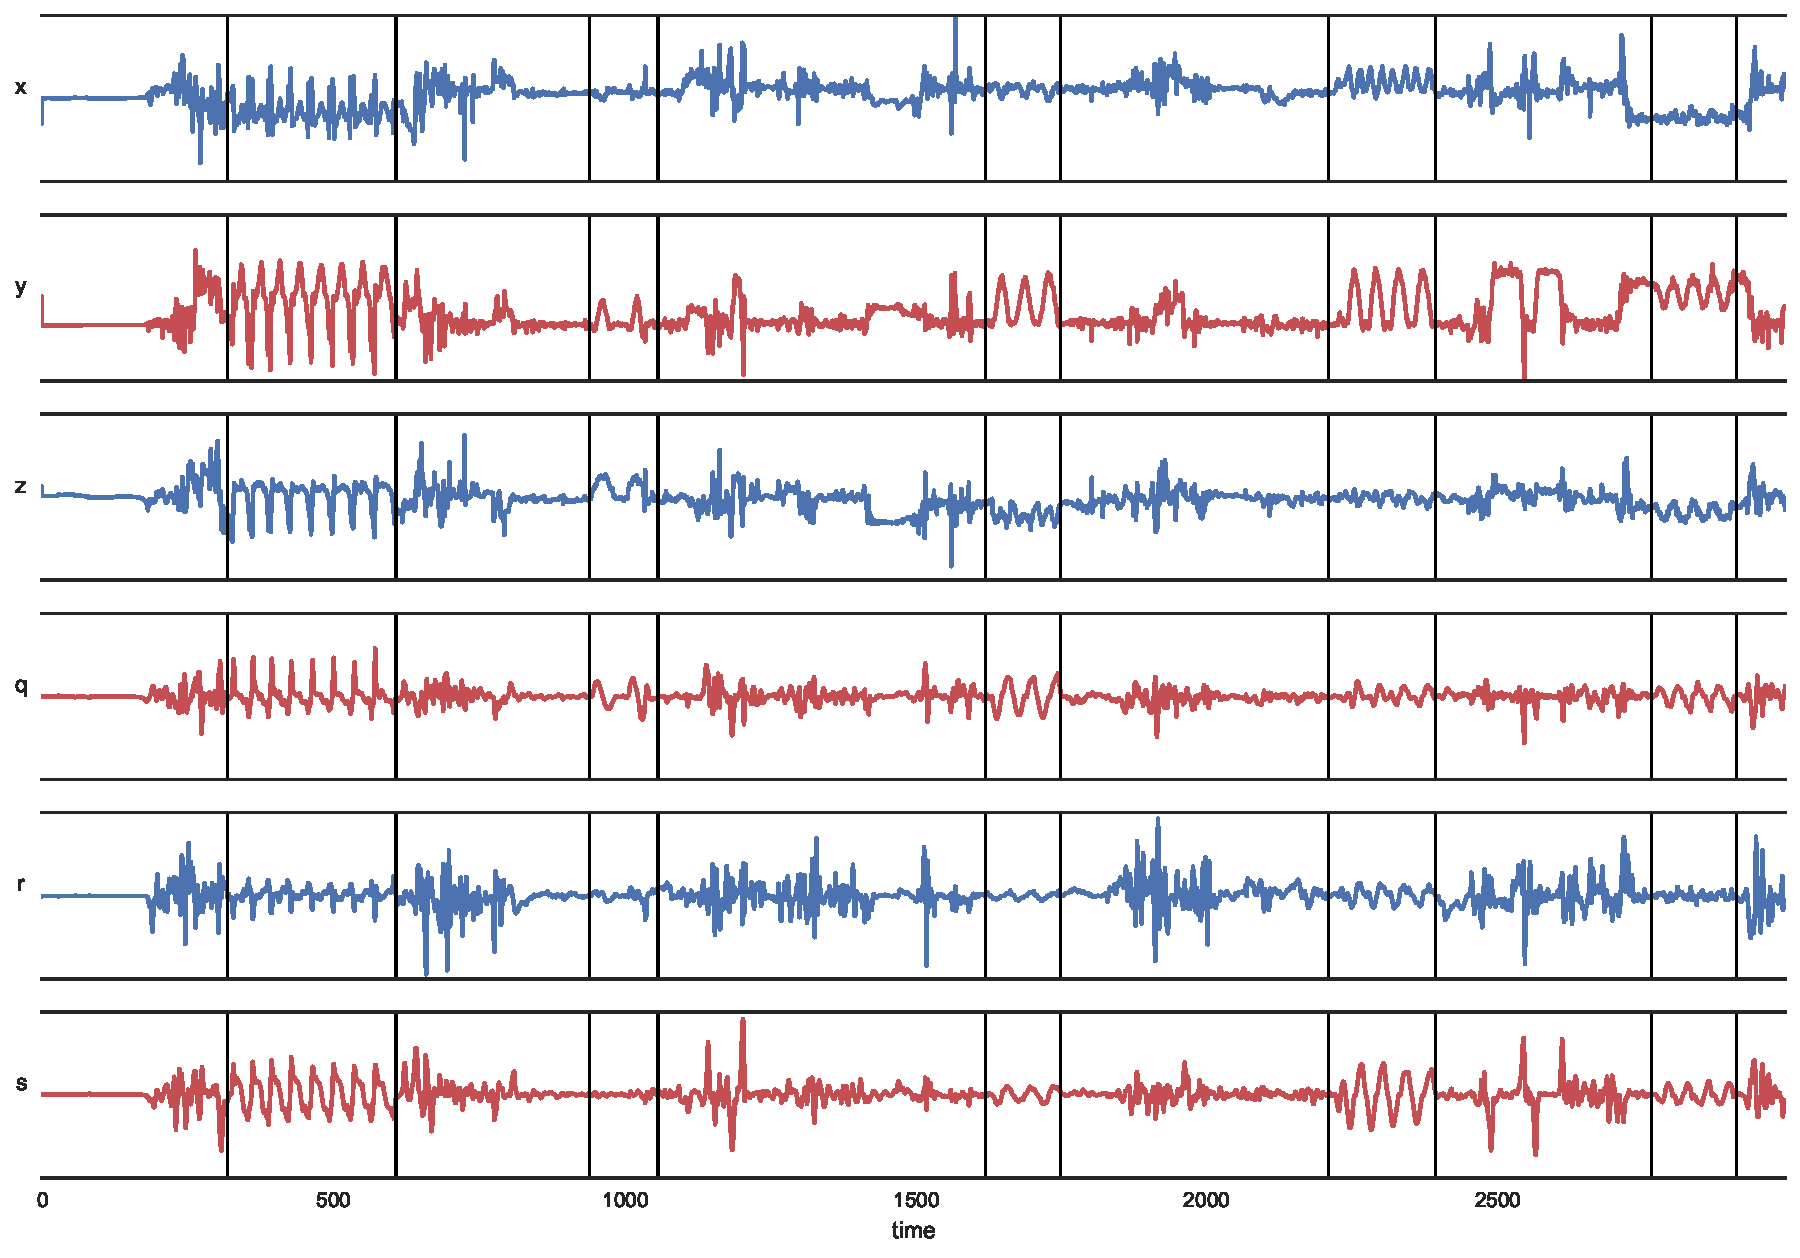
\includegraphics[width=1\textwidth]{img/routine_380.pdf}
    \caption{Example routine time series, 
    vertically order by $x$, $y$, $z$ (accelerometer, axis range from -3 to 3) 
    and $q$, $r$, $s$ (gyroscope, axis range from -600 to 600).}
    \label{fig:routine}
\end{figure}

\section{Exercise Taxonomy}
Exercise names are often ambiguous; several names can refer to the same exercise, 
and the same name can refer to different variations of the same exercise. 
The first type of naming ambiguity (many to one) is easily solved by defining a fixed reference name 
which is always used, but the second type (one to many) is more difficult to handle. 
\\\\
The second type of ambiguity typically involves positioning, resulting in exercises that are visually similar
but whose sensor readings can be drastically different. 
Examples include supinated (underhand) vs pronated (overhand) for pull-ups and dumbbell curls,
or hands on temple vs hands behind head vs arms crossed for sit-ups and crunches. To solve this problem 
we defined a standard naming convention for exercises which include form variations. This allows grouping
form variations into different classes, which was found to be beneficial for some classifiers. 
The final naming convention we adopted is
\[
    \m{[modifier] [equipment] <exercise> [(form variation)]}
\]
where square brackets and angle brackets denote optional and required arguments respectively. 
This convention results in exercise names such as
\[
    \underbrace{\text{alternating}}_{\text{modifier}} \; \underbrace{\text{dumbbell}}_{\text{equipment}} \; \underbrace{\text{bicep curl}}_{\text{exercise}} \; \underbrace{\text{(start with wrist facing forward)}}_{\text{form variation}}
\]
and
\[
    \underbrace{}_{\text{modifier}} \; \underbrace{}_{\text{equipment}} \; \underbrace{\text{pull-up}}_{\text{exercise}} \; \underbrace{\text{(supinated)}}_{\text{form variation}}
\]

\section{Technological Limitations}
The need for precise temporal synchronization between the wrist worn device and software
used to annotate the sensor data with start/stop times and repetitions end times was a significant
challenge.
\begin{itemize}
    \item BLE isn't fast enough to sync
    \item Noisy start/stop tags
    \item Noisier repetition tags (unusable)
    \item Motivation for generative model, model latent repetitive structure
\end{itemize}

\begin{figure}[t!]
    \centering
    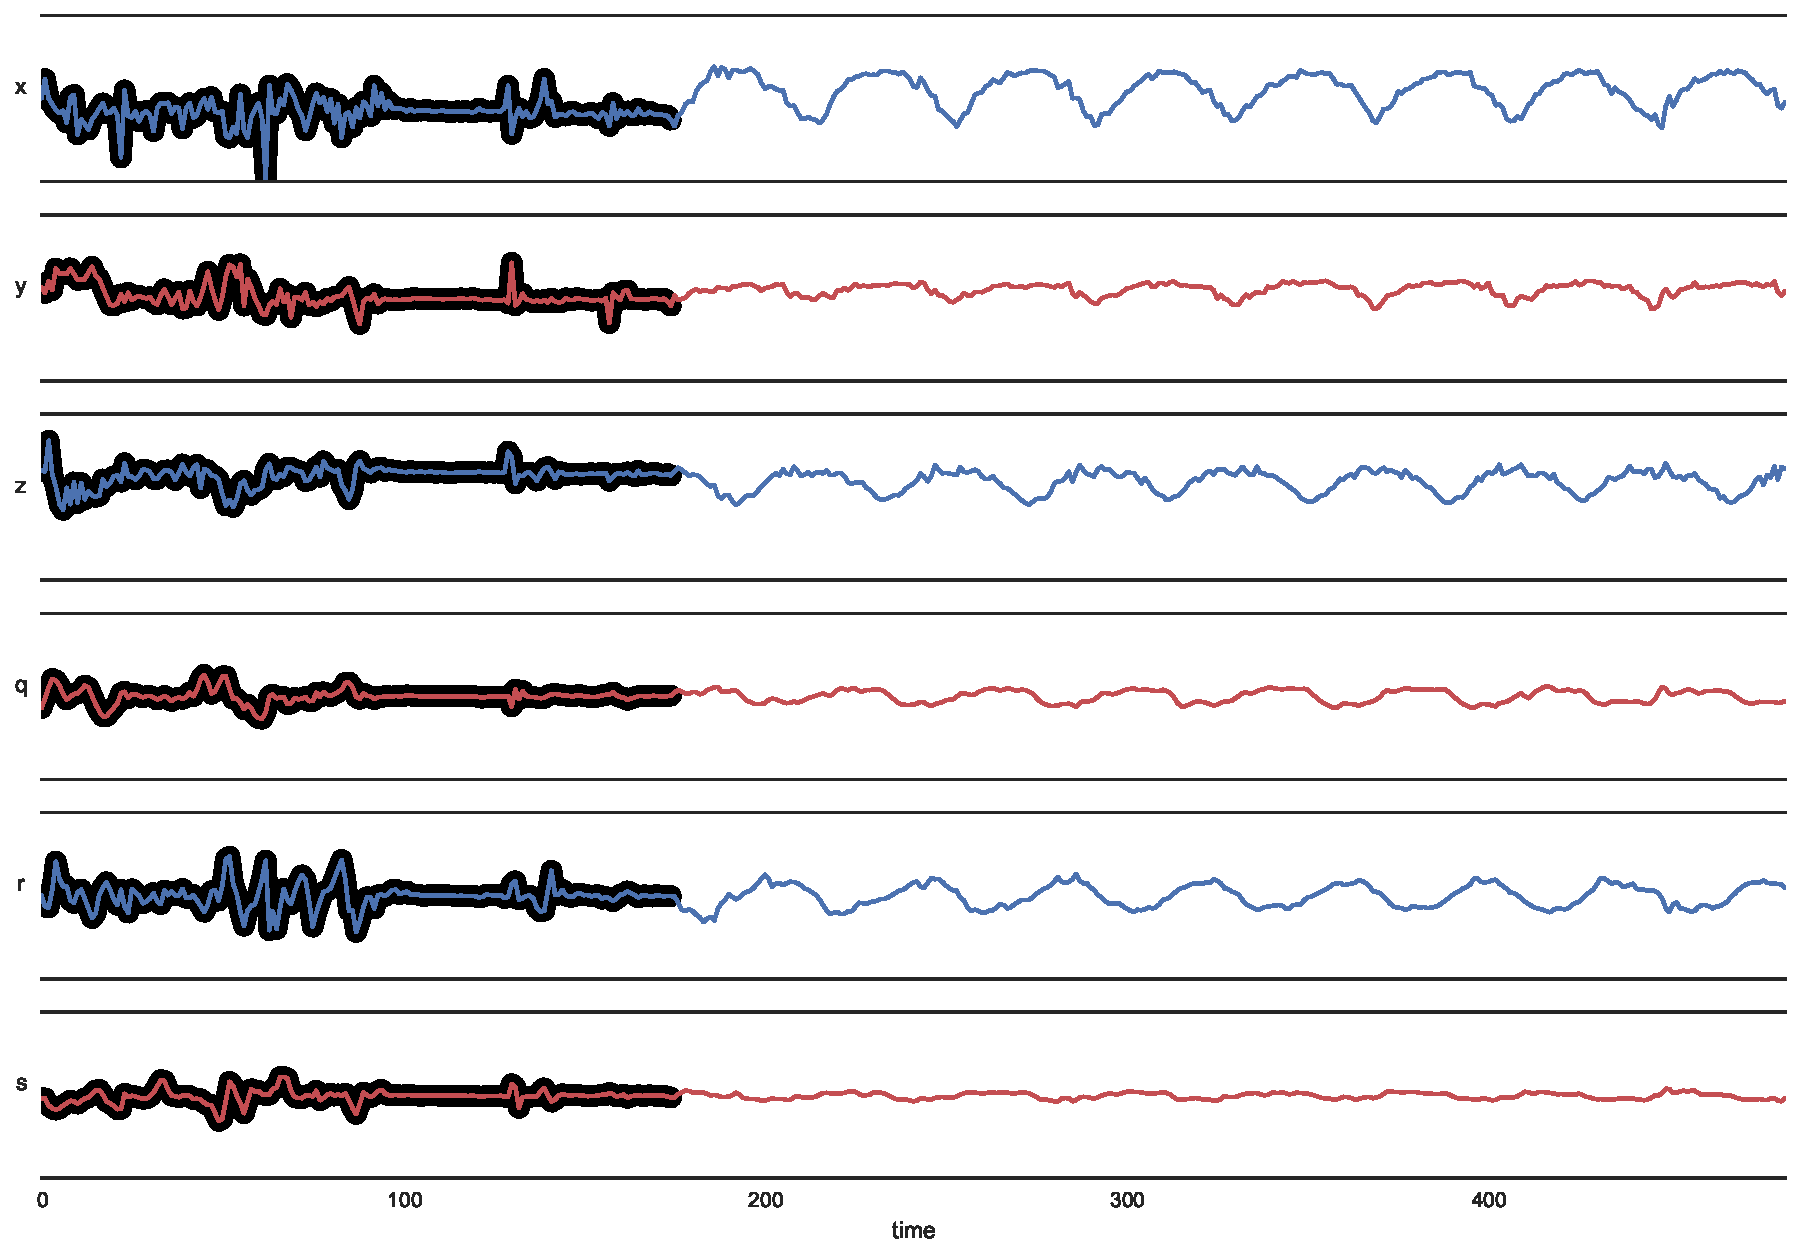
\includegraphics[width=1\textwidth]{img/annot_error_activity_202928.pdf}
    \caption{Example annotation error.}
    \label{fig:annot-arror}
\end{figure}

\chapter{Hidden Markov Models}
\acp{HMM} \cite{rabiner-hmms} are a common theme throughout this thesis. 
In the spirit of self containment this chapter introduces common terminology, 
methods and inference algorithms employed when working with \acp{HMM}. In particular
the focus is on Bayesian methods. For a more standard introduction see Kevin Murphy's excellent thesis 
\cite{murphy-thesis}, which also discusses the more general class of probabilistic models 
known as \acp{DBN}, of which \acp{HMM} and the popular Kalman filter \cite{kalman-filter}, are a member.

\section{Notation}
Standard notation used throughout is reviewed here.
Random variables are denoted by uppercase letters $X$, $Y$ 
and the values these variables take by the corresponding lower case 
letter $x$, $y$. The probability that a particular random variable $X$
takes a value $x$ is denoted by $P(X=x)$. When clear from context the uppercase
letter will be omitted and the previous expression will simply be written
$P(x)$. If $X$ has distribution $\SomeDist$ with parameters $\theta$ we write
$X \sim \SomeDist(\theta)$. The Uniform, Bernoulli, Categorical, Dirichlet, and Normal distribution
are denoted by $\Unif$, $\Bern$, $\Cat$, $\Dir$, and $\Norm$ respectively.
\\\\
As this thesis deals almost exclusively with time series, $t$ will always
be used as a time index and $T$ as the length of the time series. 
A sequence from time $t_1$ to $t_2$ is denoted by 
$\seq{x}{t_1}{t_2} = (x_{t_1}, x_{t_1 + 1}, \ldots, x_{t_2})$.
Following this notation the entire sequence is denoted $\seq{x}{1}{T}$.

\section{Introduction to Hidden Markov Models}\label{sec:hmm-intro}
\acp{HMM} are probabilistic state-space models for sequential data.
The states in an \ac{HMM} are members of a finite discrete set, and 
can be partitioned into a set of observed variables $X$, and latent 
(unobserved) variables $Y$. The latent variables evolve according to
a first order Markov process:

\[
    P(y_t \mid \seq{y}{1}{t-1}) = P(y_t \mid y_{t-1})
\]

i.e., the latent state at time $t$ depends only on the latent state 
at time $t-1$. Generalization to higher order dependencies is straightforward.
It is typically assumed that the observation at time $t$ is conditionally 
independent of all other variables given the latent variable at time $t$, 

\[
    P(x_t \mid \seq{y}{1}{T}) = P(x_t \mid y_t).
\]

Again, this assumption can be relaxed in obvious ways \cite{autoregressive-shannon}.
For ease of exposition the simplest formulation presented above is used here.
\\\\
Given the above assumptions the joint probability of a sequence of observations 
$\seq{x}{1}{T}$ and latent states $\seq{y}{1}{T}$ is given by

\begin{equation}\label{eq:hmm-joint}
    P(\seq{x}{1}{T}, \seq{y}{1}{T}) = 
    P(y_1)P(x_1 \mid y_1) \prod_{t=2}^T P(y_t \mid y_{t-1}) P(x_t \mid y_t).
\end{equation}

The corresponding generative story is given by

\begin{enumerate}
    \item Sample an initial state $y_1 \sim \Cat(\pi_0)$.
    \item Sample an initial observation $x_t \sim \SomeDist(\phi_{y_1})$.
    \item For $t = 2$ to $T$
    \begin{enumerate}
        \item Sample the next state $y_{t} \mid z_t \sim \Cat(\pi_{y_{t-1}})$ conditioned on the previous state.
        \item Sample the next observation $x_t \mid y_t \sim \SomeDist(\phi_{y_t})$ conditioned on the current state.
    \end{enumerate}
\end{enumerate}

where $\SomeDist$ is some parametric emission distribution.
Dependencies can be visualized graphically in Figure (\ref{fig:hmm}), 
where vertices represent variables, edges represent dependencies, 
and grey vertices represent observed variables.

\begin{figure}[ht!]
    \centering
    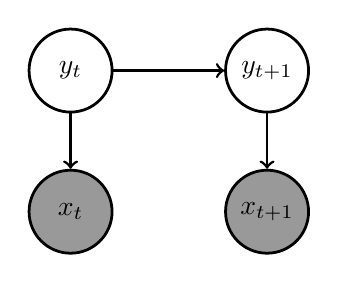
\begin{tikzpicture}
        \node[randvar] (y_t) {$y_t$};
        \node[randvar,fill=grey3,below=20pt of y_t] (x_t) {$x_t$};

        \node[randvar,right=40pt of y_t] (y_tp1) {$y_{t+1}$};
        \node[randvar,fill=grey3,below=20pt of y_tp1] (x_tp1) {$x_{t+1}$};

        \draw[->,line width=1pt] (y_t) to (y_tp1);
        \draw[->,line width=1pt] (y_t) to (x_t);
        \draw[->,line width=1pt] (y_tp1) to (x_tp1);
    \end{tikzpicture}
    \caption{Slice representation of an \ac{HMM}.}
    \label{fig:hmm}
\end{figure}

\subsection{Inference}
This Section outlines two useful algorithms for \acp{HMM} 
assuming a fixed set of parameters. The first computes the 
likelihood of an observed sequence under the given parameters. 
The second computes the most likely sequence of states given
an observed sequence. The number of states in the \ac{HMM} will
be denoted by $K$.

\subsubsection{Likelihood}
Computing the likelihood of an observed sequence $\seq{x}{1}{T}$ can be done naively
by marginalizing of all possible length $T$ states sequences

\[
    P(\seq{x}{1}{T}) = \sum_{\seq{y}{1}{T}} P(\seq{x}{1}{T}, \seq{y}{1}{T})
\]

Computation in this manner requires time $O(TK^T)$ and is infeasible for all
but the smallest $K$ and $T$. A more efficient algorithm exists requiring only time
$O(TK^2)$. It is typically referred to as the forward, alpha, or 
simply sum-product algorithm in the more general context of \acp{PGM}.
\\\\
Define $\alpha_{t,y_t} = P(y_t, \seq{x}{1}{t})$ as the joint probability
of the state at time $t$ being $y_t$ and the entire observation sequence up to
time $t$. The key insight is that $\alpha_{t,*}$ may be computed recursively 
from $\alpha_{t-1,*}$ as

\begin{align*}
    \alpha_{t,y_t}
    &= P(y_t, \seq{x}{1}{t}) \\
    &= P(x_t \mid y_t) \sum_{y_{t-1}} P(y_t \mid y_{t-1}) P(y_{t-1}, \seq{x}{1}{t-1}) \\
    &= P(x_t \mid y_t) \sum_{y_{t-1}} P(y_t \mid y_{t-1}) \alpha_{t-1,y_{t-1}} \\
\intertext{with the base case given by}
    \alpha_{1,y_1} &= P(y_1)P(x_1 \mid y_1)\\
\end{align*}

It follows that 

\[
    P(\seq{x}{1}{T}) = \sum_{y_T} P(y_T, \seq{x}{1}{T}) = \sum_{y_T} \alpha_{T,y_T}.
\]

\subsubsection{The \ac{MAP} State Sequence}
The algorithm for efficiently computing the most likely state sequence given an 
observed sequence is closely related to the algorithm for computing the likelihood 
of an observed sequence discussed above. 
It is commonly referred to as the Viterbi or max-product algorithm.
\\\\
Define 

\[
    v_{t,i} = \max_{\seq{y}{1}{t}}\{P(\seq{x}{1}{t}, \seq{y}{1}{t}) \mid y_t = i\}
\] 

as the probability of the most likely sequence of $t$ states ending in state $i$ 
given $\seq{x}{1}{t}$. Then $v_{t,*}$ may be computed recursively from $v_{t-1,*}$ as

\begin{align*}
    v_{t,y_t} 
    &= \max_{y_{t-1}}\{ P(x_{t} \mid y_t) P(y_t \mid y_{t-1}) v_{t-1,y_{t-1}} \} \\
    &= P(x_t \mid y_t) \max_{y_{t-1}}\{ P(y_t \mid y_{t-1}) v_{t-1,y_{t-1}} \} \\
\intertext{with the base case given by}
    v_{1,y_1} &= P(y_1)P(x_1 \mid y_1).
\end{align*}

The most likely path is easily recovered by storing a $T \times K$ table of back pointers 
whose $t,k$ entry is the most likely state leading to state $k$ at time $t$.

\section{The Bayesian Approach}
Bayesian statistics treats quantities of interest as random variables. 
In the context of Machine Learning, Bayesian methods are frequently used 
for parameter estimation and model selection, although only the former is 
considered here. The Bayesian approach to parameter estimation begins by 
defining a prior distribution over model parameters before observing any data, 
$P(\theta)$. After observing data $D$ one is typically interested in the 
posterior, i.e., the probability distribution over parameters, conditioned on observing
$D$.

\[
    P(\theta \mid D) = \frac{P(\theta)P(D \mid \theta)}{P(D)}.
\]

The term $P(D \mid \theta)$ appearing above is referred to as the likelihood.
Using this terminology one is able to write
\[
    \text{Posterior} \propto \text{Prior} \times \text{Likelihood}.
\]

\subsection{The Dirichlet-Categorical Distribution}
The Dirichlet distribution is a probability distribution defined on the $K-1$ 
dimensional simplex $\triangle$. $\pi \in \triangle \implies \pi_k > 0$, $\sum_k \pi_k = 1$.
It is useful to conceptualize the Dirichlet distribution as a distribution over
parameters of Categorical or Multinomial distributions. From this point of view 
samples from a Dirichlet distribution are themselves probability distributions.
\\\\
If $\pi \sim \Dir(\alpha)$ then

\begin{equation}
    P(\pi) = \frac{1}{\Bf(\alpha)} \prod_k \pi_k^{\alpha_k-1}, \label{eq:dir-pdf}
\end{equation}

where $\Bf$ is the multivariate beta function,

\begin{equation}
    \Bf(\alpha) = \frac{\prod_k \Gamma(\alpha_k)}{\Gamma(\sum_k \alpha_k)}, \label{eq:betafunc}
\end{equation}

and $\Gamma$ is the generalized factorial.
\\\\
Let $D = \{x_1, \ldots, x_m\}$ and $n_k = \sum_{x \in D} \1\{x = k\}$ count 
the number of occurrences of $k \in D$. Assuming

\begin{align*}
    \pi & \sim \Dir(\alpha) \\
    x_i & \sim \Cat(\pi),\; i = 1, \ldots, m.
\end{align*}

Then

\begin{align*}
    P(\pi \mid D, \alpha) 
    &= \frac{P(\pi \mid \alpha) P(D \mid \pi, \alpha)}{P(D)} \\
    & \propto P(\pi \mid \alpha) P(D \mid \pi) \\
    &= \frac{1}{\Bf(\alpha)} \prod_k \pi_k^{\alpha_k - 1} \prod_k \pi_k^{n_k} \\
    &= \frac{1}{\Bf(\alpha)} \prod_k \pi_k^{n_k + \alpha_k - 1},
\end{align*}

The Dirichlet distribution is referred to as the \emph{conjugate} prior for the 
Categorical distribution since the posterior $P(\pi \mid D, \alpha)$ and prior $P(\pi \mid \alpha)$ 
have the same form \cite{gelman-bayesian-data-analysis}. The marginal likelihood $P(D \mid \alpha)$ 
can be obtained by integrating over $\pi$ as follows.

\begin{align}
    P(D \mid \alpha) 
    &= \int_{\triangle} P(\pi \mid \alpha)\prod_{x \in D} P(x \mid \pi) d \pi \nonumber \\
    % 
    &= \int_{\triangle} \frac{\Gamma(\sum_k \alpha_k)}{\prod_k \Gamma(\alpha_k)}
                        \prod_k \pi^{\alpha_k - 1}_k \prod_k \pi_k^{n_k} d \pi \nonumber \\
    % 
    &= \frac{1}{\Bf(\alpha)}
       \int_{\triangle} \prod_k \pi_k^{n_k + \alpha_k - 1} d \pi. \label{eq:unnormed-dir}
\end{align}

The term inside the integral in (\ref{eq:unnormed-dir}) is the unnormalized probability density function
of a Dirichlet distribution with parameters $n_k + \alpha_k$. Since (\ref{eq:dir-pdf})
is a pdf it follows that

\begin{align}
    1 
    &= \int_\triangle \frac{1}{\Bf(\bm{n} + \alpha)} \prod_k \pi_k^{n_k + \alpha_k - 1} d \pi \nonumber \\
    &= \frac{1}{\Bf(\bm{n} + \alpha)} \int_\triangle \prod_k \pi_k^{n_k + \alpha_k - 1} d \pi \nonumber  \\
\implies \Bf(\bm{n} + \alpha) &= \int_\triangle \prod_k \pi_k^{n_k + \alpha - 1} d \pi \label{eq:dir-int-sol}
\end{align}

where $\bm{n} = (n_1, \ldots, n_K)$ is the vector of counts defined above.
Plugging (\ref{eq:dir-int-sol}) into (\ref{eq:unnormed-dir}) yields

\begin{equation}
    P(D \mid \alpha) 
    = \frac{1}{\Bf(\alpha)}\int_{\triangle} \prod_k \pi_k^{n_k + \alpha_k - 1} d \pi
    = \frac{\Bf(\bm{n} + \alpha)}{\Bf(\alpha)}. \label{eq:dpcmarg}
\end{equation}

The process of marginalizing over a parameter as above is common in Bayesian analysis. 
It is particularly helpful in the context of Gibbs sampling since reducing the number
of parameters that need to be sampled frequently results in increased efficiency.

\subsection{The Bayesian Hidden Markov Model}
In the context of \acp{HMM}, it is convenient due to conjugacy to place Dirichlet priors
with parameters $\alpha_0$ and $\alpha_i$ over the initial and transition 
parameters $\pi_0$ and $\pi_i$. Assuming each state's emission distribution is also Categorical 
with parameters $\theta_i$, a Dirichlet prior with parameters $\alpha_i^\p$ may be placed 
over these parameters as well. This results in the following generative story.

\begin{align*}
    \pi_0 & \sim \Dir(\alpha_0) \\
    \pi_i & \sim \Dir(\alpha_i),\; i = 1, \ldots, \abs{Y} \\
    \theta_i & \sim \Dir(\alpha_i^\p),\; i = 1, \ldots, \abs{Y} \\ 
    y_1 & \sim \Cat(\pi_0) \\
    y_{t+1} \mid y_t & \sim \Cat(\pi_{y_t}),\; t = 1, \ldots, T-1 \\
    x_t \mid y_t & \sim \Cat(\theta_{y_t}), \; t = 1, \ldots, T.
\end{align*}

Let $(\mathcal{X}, \mathcal{Y}) = (\{\seq{x}{1}{T_1}^1, \ldots, \seq{x}{1}{T_m}^m\},  
\{\seq{y}{1}{T_1}^1, \ldots, \seq{y}{1}{T_m}^m\})$ be a set of
observation and corresponding state sequences, and

\begin{align*}
    n_{0, i} &= \sum_{y \in \mathbf{y}} \1\{y_1 = i\} \\
    n_{i, j} &= \sum_{y \in \mathbf{y}} \sum_{t} \1\{y_{t-1} = i \wedge y_t = j\} \\
    n_{i, o}^\p &= \sum_{(\seq{x}{1}{T},\seq{y}{1}{T}) \in (\mathcal{X},\mathcal{Y})} \sum_{t} \1\{y_t = i \wedge x_t = o\} \\
\end{align*}

count the number of times the initial states is $i$, the number of transition from state $i$ to $j$,
and the number of times a particular observation $o$ is observed in state $i$ respectively. Then 

\begin{align}  \label{eq:bayes-hmm-joint-simple}
 P(\mathcal{X}, \mathcal{Y} \mid \Theta, \alpha) 
 &=  P(\pi_0 \mid \alpha_0) \prod_i P(\pi_i \mid \alpha_i) \prod_i P(\theta_i \mid \alpha^\prime) \nonumber\\
 & \times \prod_{(\seq{x}{1}{T},\seq{y}{1}{T}) \in (\mathcal{X},\mathcal{Y})} P(\seq{x}{1}{T},\seq{y}{1}{T})
\end{align}

where $\Theta = \{\pi_0, \pi_i, \theta_i\}$ and $\alpha = \{alpha_0, \alpha_i, \alpha_i^\prime\}$.

Substituting into (\ref{eq:bayes-hmm-joint-simple}) the form of the priors and 
rewriting in terms of the counting variables gives

\begin{align} \label{eq:bayes-hmm-joint-full}
    P(\mathcal{X}, \mathcal{Y} \mid \Theta, \alpha)
    &= \frac{1}{\Bf(\alpha_0)} \prod_{i} \pi_{0,i}^{n_{0,i} + \alpha_{0,i} - 1} \nonumber \\
    & \times \prod_i \left(\frac{1}{\Bf(\alpha_i)} \prod_{j} \pi_{i,j}^{n_{i,j} + \alpha_{i,j} - 1}\right) \nonumber \\
    & \times \prod_i \left(\frac{1}{\Bf(\alpha_i^\prime)} \prod_{v} \pi_{i,j}^{n_{i,v}^\prime + \alpha_{i,v}^\prime - 1}\right)
\end{align}

Repeatedly applying the same steps used to derive (\ref{eq:dir-int-sol})
allows one to write the marginal joint probability of $(\mathcal{X}, \mathcal{Y})$
in terms of hyperparameters and counts.

\begin{equation}
    P(\mathcal{X}, \mathcal{Y} \mid \alpha_0, \alpha_i, \alpha_i^\prime)
    = \frac{\Bf((\bm{n}_0 + \alpha_0)}{\Bf(\alpha_0)}
    \prod_i \frac{\Bf{(\bm{n}_i + \alpha_i}}{\Bf(\alpha_i)} 
    \frac{\Bf((\bm{n}_i^\p + \alpha_i^\p)}{\Bf(\alpha_i^\p)} 
    \label{eq:marg-likelihood-hmm}
\end{equation}

where the counts have been extended to vectors as was done previously,

\begin{align*}
    \bm{n}_0 &= (n_{0,1}, \ldots, n_{0,\abs{Y}}) \\
    \bm{n}_i &= (n_{i,1}, \ldots, n_{i,\abs{Y}}),\; i = 1, \ldots, \abs{Y} \\
    \bm{n}_i^\p &= (n_{i,1}^\p, \ldots, n_{i,\abs{X}}^\p),\; i = 1, \ldots, \abs{Y}. \\
\end{align*}

From an algorithmic perspective (\ref{eq:marg-likelihood-hmm}) has a particularly convenient
form. Given the counting variables the time required to compute the marginal likelihood does not 
depend on the number of sequences or their length, only the number of states and and possible observations.

\begin{figure}[ht!]
    \centering
    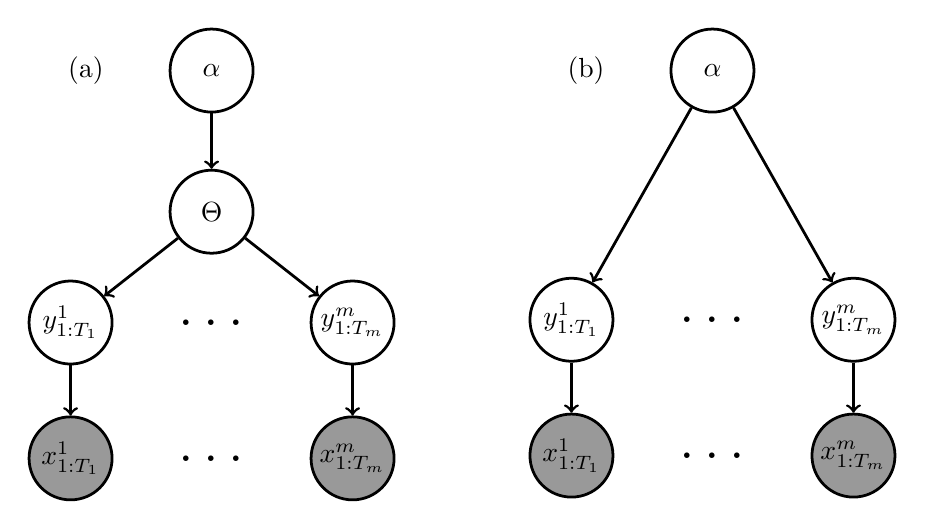
\begin{tikzpicture}
        \node[randvar] (alpha) {$\alpha$};
        \node[textbox,left=20pt of alpha] (a) {\normalsize{(a)}};
        \node[randvar,below=20pt of alpha] (Theta) {$\Theta$};
        \node[textbox,below=20pt of Theta] (ydots) {\huge{$\ldots$}};
        \node[randvar,left=20pt of ydots] (y1) {$\seq{y}{1}{T_1}^1$};
        \node[randvar,right=20pt of ydots] (ym) {$\seq{y}{1}{T_m}^m$};
        \node[textbox,below=40pt of ydots] (xdots) {\huge{$\ldots$}};
        \node[randvar,fill=grey3,left=20pt of xdots] (x1) {$\seq{x}{1}{T_1}^1$};
        \node[randvar,fill=grey3,right=20pt of xdots] (xm) {$\seq{x}{1}{T_m}^m$};

        \node[randvar,right=150pt of alpha] (alpha-marg) {$\alpha$};
        \node[textbox,left=20pt of alpha-marg] (b) {\normalsize{(b)}};
        \node[textbox,below=70pt of alpha-marg] (ydots-marg) {\huge{$\ldots$}};
        \node[randvar,left=20pt of ydots-marg] (y1-marg) {$\seq{y}{1}{T_1}^1$};
        \node[randvar,right=20pt of ydots-marg] (ym-marg) {$\seq{y}{1}{T_m}^m$};
        \node[textbox,below=40pt of ydots-marg] (xdots-marg) {\huge{$\ldots$}};
        \node[randvar,fill=grey3,left=20pt of xdots-marg] (x1-marg) {$\seq{x}{1}{T_1}^1$};
        \node[randvar,fill=grey3,right=20pt of xdots-marg] (xm-marg) {$\seq{x}{1}{T_m}^m$};

        \draw[->,line width=1pt] (alpha) to (Theta);
        \draw[->,line width=1pt] (Theta) to (y1);
        \draw[->,line width=1pt] (Theta) to (ym);
        \draw[->,line width=1pt] (y1) to (x1);
        \draw[->,line width=1pt] (ym) to (xm);

        \draw[->,line width=1pt] (alpha-marg) to (y1-marg);
        \draw[->,line width=1pt] (alpha-marg) to (ym-marg);
        \draw[->,line width=1pt] (y1-marg) to (x1-marg);
        \draw[->,line width=1pt] (ym-marg) to (xm-marg);
    \end{tikzpicture}
    \caption{Graphical representation of a Bayesian \ac{HMM} without (a) and with (b)
    marginalization of the parameters $\Theta$. Notice that marginalization
    of $\Theta$ introduces dependencies between latent states $y$, since
    they now share a common parent $\alpha$ in (b).}
    \label{fig:hmm-marg}
\end{figure}

\section{A Block Collapsed Gibbs Sampler for Hidden Markov Models} \label{sec:collapsed-sampler}
This Section develops a collapsed Gibbs Sampler for $P(\mathcal{Y} \mid \mathcal{X}, \alpha)$.
We do so using a block-wise approach, resampling an entire state sequence $\seq{y}{1}{T}^i$ given
$\mathcal{X}$, $\mathcal{Y}_{-i}, \alpha$, where $\mathcal{Y}_{-i}$ denotes 
$\mathcal{Y} \setminus \{\seq{y}{1}{T}^i\}$. This sampler follows the approach 
described in \cite{pcfg-bayesian-johnson} for \acp{PCFG}, and utilized 
for \acp{HMM} in \cite{hmm-comparison-johnson}. 
\\\\
The primary difficulty in constructing such a sampler is due to marginalizing over the parameters,
as doing so introduces dependencies amongst the latent state sequences $\mathcal{Y}$, Figure (\ref{fig:hmm-marg}). 
Let us proceed in the usual manner for constructing such a Gibbs sampler. We have 

\begin{equation}
    P(\seq{y}{1}{T}^i \mid \mathcal{Y}_{-i}, \mathcal{X}, \alpha) 
    = \frac{P(\seq{x}{1}{T}^i \mid \seq{y}{1}{T}^i)P(\seq{y}{1}{T}^i \mid \mathcal{Y}_{-i}, \mathcal{X}_{-i}, \alpha)}
      {P(\seq{x}{1}{T}^i \mid \mathcal{Y}_{-i}, \mathcal{X}_{-i}, \alpha)}. \label{eq:hmm-gibbs-problem}
\end{equation}

The $P(\seq{x}{1}{T}^i \mid \mathcal{Y}_{-i}, \mathcal{X}_{-i}, \alpha)$ term in the denominator 
of (\ref{eq:hmm-gibbs-problem}) is particularly problematic, as noted by \cite{pcfg-bayesian-johnson}. 
The need to marginalize over all possible state sequences (without reference to a set of \ac{HMM} parameters) 
is particularly difficult, and it is not clear how one would approach such a problem
in a computationally efficient manner.
\\\\
Instead, since the denominator of (\ref{eq:hmm-gibbs-problem}) does not depend on $\seq{y}{1}{T}^i$, 
we can appeal to a Metropolis-Hastings approach, knowing this troublesome term will cancel when 
computing the acceptance probability. 
\\\\
A Metropolis-Hastings sampler \cite{mcmc-ml} is a popular \ac{MCMC} algorithm for drawing samples
from a target distribution $P(X)$, provided one is able to compute a value
$f(x)$ such that $f(x) \propto P(x)$. The sampler works by repeatedly drawing a 
sample $x^*$ from a proposal distribution $q(\cdot \mid x)$ which is probabilistically
accepted, replacing the current $x$, or rejected. The result is a series of samples 
whose stationary distribution is $P(X)$. In the special case that the proposal distribution
does not depend on the current sample, $q(x^* \mid x) = q(x^*)$, the proposal is said to 
be \emph{independent}. The generic Metropolis-Hastings algorithm is given in algorithm (\ref{alg:mh-generic}).

\begin{algorithm}[H]
    \caption{The Metropolis-Hastings Algorithm.\label{alg:mh-generic}}
    \begin{algorithmic}[1]
        \Require{$x^0$ starting value}
        \For{$i \gets 1, \ldots, n$}
            \State $x^* \sim q(\cdot \mid x^{i-1})$
            \State $u \sim \Unif(0, 1)$
            \If{$u < \dfrac{f(x^*) q(x^{i-1} \mid x^*)}{f(x^i) q(x^* \mid x^{i-1})}$}
                \State $x^i \gets x^*$
            \Else
                \State $x^i \gets x^{i-1}$
            \EndIf
        \EndFor
        \State \Return{$(x^1, \ldots, x^n)$}
    \end{algorithmic}
\end{algorithm}

For the problem of sampling a state sequence $\seq{y}{1}{T}$, the Metropolis-Hastings algorithm
is utilized as a subroutine to sample from the conditional distribution required
by the Gibbs sampler. This is known as Metropolis-within-Gibbs \cite{mh-within-gibbs}. 
Let $\mathcal{Y}^* = \{\seq{y}{1}{T}\}^* \cup \mathcal{Y}_{-i}$, 
where $\seq{y}{1}{T}^*$ is drawn from some an independent distribution $q(\cdot)$. 
Then the proposed $\seq{y}{1}{T}^*$ is accepted with probability
\begin{align}
    p
    &= \frac{P(\seq{y}{1}{T}^* \mid \mathcal{Y}_{-i}, \mathcal{X}, \alpha)}
            {P(\seq{y}{1}{T}^i \mid \mathcal{Y}_{-i}, \mathcal{X}, \alpha)} \
            \frac{q(\seq{y}{1}{T}^i)}{q(\seq{y}{1}{T}^*)} \nonumber \\
    &= \frac{P(\mathcal{Y}^*, \mathcal{X} \mid \alpha)}
            {P(\mathcal{Y}, \mathcal{X} \mid \alpha)}
            \frac{q(\seq{y}{1}{T}^i)}{q(\seq{y}{1}{T}^i*)} \nonumber \\
    &= \frac{\Bf(\bm{n}_0^* + \alpha_0)}
            {\Bf(\bm{n}_0 + \alpha_0)} 
    \prod_j \left[ \frac{\Bf(\bm{n}_j^* + \alpha_j)}
                        {\Bf(\bm{n}_j + \alpha_j)} 
                   \frac{\Bf(\bm{n}_j^{\prime *} + \alpha_j^\p)}
                        {\Bf(\bm{n}_j^\p + \alpha_j^\p)}\right] 
                   \frac{q(\seq{y}{1}{T}^i)}{q(\seq{y}{1}{T}^*)} \label{eq:mh-hmm-prob-accept}
\end{align}

where the $\bm{n}^*$ are analogous to the $\bm{n}$ terms, but contain the 
counts from the proposal $\seq{y}{1}{T}^*$ rather than $\seq{y}{1}{T}^i$.
\\\\
The proposal distribution $q(\cdot)$ is itself a \ac{HMM} with parameters 
$\hat{\Theta} = \{\hat{\pi}_0, \hat{\pi}_i, \hat{\theta}_i\}$ derived from the current 
$\mathcal{Y}_{-i}$, $\mathcal{X}_{-i}$. In particular $\hat{\Theta}$ is set to its expected value,
$\hat{\Theta} = \E[\Theta \mid Y_{-i}, X_{-i}, \alpha]$, and then the proposal is sampled from

\[
    \seq{y}{1}{T}^* \sim P(\cdot \mid \seq{x}{1}{T}^i, \hat{\Theta})
\]
utilizing the algorithm outlined in \cite{scott-bayesian-hmm}.
\\\\
\textbf{TODO:} Explain Scott's algorithm.
\\\\
Empirically this results in a majority of proposals $\seq{y}{1}{T}^*$ being accepted, which aligns
with the observations reported by \cite{hmm-comparison-johnson}.

\section{Mixtures of Hidden Markov Models}\label{sec:mohmms}
Extension to a finite mixture of $K$ \acp{HMM} is straightforward and results
in the following generative story

\begin{align*}
    \phi & \sim \Dir(\beta) \\
    \pi_{k,0} & \sim \Dir(\alpha_0), k=1,\ldots,K \\
    \pi_{k,i} & \sim \Dir(\alpha_i),\; k=1,\ldots,K,\; i=1,\ldots,\abs{Y} \\
    \theta_{k,i} & \sim \Dir(\alpha_i^\p),\; k=1,\ldots,K,\; i = 1,\ldots,\abs{Y} \\
    z & \sim \Cat(\phi) \\
    \seq{x}{1}{T}, \seq{y}{1}{T} \mid z & \sim \HMM(\Theta_z).
\end{align*}

where $\HMM(\Theta_{z_i})$ is used as shorthand for the \ac{HMM}
generative story outlined in Section \ref{sec:hmm-intro}. Again, the marginal likelihood
$\mathcal{Z}$, $\mathcal{Y}$, and $\mathcal{X}$ can be expressed in closed form in terms of 
hyper parameters and counts.

\begin{multline}
    P(\mathcal{Z}, \mathcal{X}, \mathcal{Y} \mid \alpha, \beta) = \\
    \frac{\Bf(\bm{c} + \beta)}{\Bf(\beta)}
    \prod_k
    \left(
        \frac{\Bf(\bm{n}_{k,0} + \alpha_0)}{\Bf(\alpha_0)} 
        \prod_i 
        \left(
            \frac{\Bf(\bm{n}_{k,i} + \alpha_i)}{\Bf(\alpha_i)} 
            \frac{\Bf(\bm{n}_{k,i}^\p + \alpha_i^\p)}{\Bf(\alpha_i^\p)}
        \right)
    \right). \label{eq:joint-marg-finite-mixture}
\end{multline}

where $c_k = \sum_{z \in \mathcal{Z}}\1\{z = k\}$ and $\bm{c} = (c_1, \ldots, c_K)$.
\\\\
In many situations $K$ is unknown. Estimation of $K$ can be carried out using standard 
techniques such as cross validation or Bayesian Information Criterion, but this is
often computationally difficult and philosophically unsatisfying. A modern 
approach to dealing with this problem is Bayesian nonparametrics \cite{jordan-bayesian-nonparam}. 
In brief, Bayesian nonparametrics allow one to sidestep the problems associated with finite
capacity models, by assuming observations are generated from infinite dimensional objects,
for which only a finite number or involved in the generation of a finite set of samples. 
\\\\
In the case of mixture models, the above model can naturally be extended to handle a 
countably infinite number of cluster components using a Dirichlet Process \cite{teh-dirichlet}.
The constructive definition of the Dirichlet process is given in terms of a 
\emph{stick-breaking process} \cite{sethuraman-constructive} with parameter 
$\beta \in \mathbb{R}_{>0}$, frequently denoted $\GEM(\beta)$.

\begin{align*}
    \xi_k & \sim \Beta(1, \beta), k = 1,\ldots,\infty\\
    \phi_k & = \xi_k \prod_{l=1}^{k-1} (1 - \xi_l)
\end{align*}

Extension of the finite mixture of \acp{HMM} to the nonparametric case thus assumes cluster 
assignments are sampled from an infinite dimensional $\phi$, itself sampled
from a $\GEM(\beta)$ distribution.

\begin{align*}
    \phi & \sim \GEM(\beta) \\
    \pi_{k,0} & \sim \Dir(\alpha_0), k=1,\ldots,\infty \\
    \pi_{k,i} & \sim \Dir(\alpha_i),\; k=1,\ldots,\infty,\; i=1,\ldots,\abs{Y} \\
    \theta_{k,i} & \sim \Dir(\alpha_i^\p),\; k=1,\ldots,\infty,\; i = 1,\ldots,\abs{Y} \\
    z & \sim \phi \\
    \seq{x}{1}{T}, \seq{y}{1}{T} \mid z & \sim \HMM(\Theta_z).
\end{align*}

Note that for any finite set of $\{z_1, \ldots, z_m\} = \mathcal{Z}$, 
$\bm{c}$ contains at most $m$ unique elements. In analogy to the finite 
mixture me, denote the number of unique elements $K$. Then the marginal likelihood 
of $\bm{c}$ given $\beta$ has the following form \cite{kyung-estimation-dirichlet}

\begin{equation}\label{dp-marg}
    P(\bm{c} \mid \beta) = \frac{m^K \Gamma(\beta)}{\Gamma(\beta + m)} \prod_k \Gamma(c_k).
\end{equation}

Collapsing all parameters results in the following slight alteration of 
equation ($\ref{eq:joint-marg-finite-mixture}$).

\begin{multline}
    P(\mathcal{Z}, \mathcal{X}, \mathcal{Y} \mid \alpha) =
    \left(\frac{m^K \Gamma(\beta)}{\Gamma(\beta + m)} \prod_k \Gamma(c_k)\right) \\
    \times \prod_k 
    \left(
        \frac{\Bf(\bm{n}_{k,0} + \alpha_0)}{\Bf(\alpha_0)} 
        \prod_i 
        \left(
            \frac{\Bf(\bm{n}_{k,i} + \alpha_i)}{\Bf(\alpha_i)} 
            \frac{\Bf(\bm{n}_{k,i}^\p + \alpha_i^\p)}{\Bf(\alpha_i^\p)}
        \right)
    \right). \label{eq:joint-marg-infinite-mixture}
\end{multline}

Having derived an expression for the the marginal likelihood of an infinite
mixture of \acp{HMM}, the same generic Metropolis-within-Gibbs approach presented
in Section \ref{sec:collapsed-sampler} could be applied to carry out inference in
the infinite mixture of \acp{HMM}. 
\\\\
However, collapsed Gibbs sampling for Dirichlet processes is a well studied problem for 
which numerous solutions exist \cite{neal-mcmc-dp}. In particular it would be easy
to alternate between sampling $z_i$ variables and latent state sequences $\seq{y}{1}{T}^i$.
Unfortunately this will mix poorly, since the cluster allocation is highly coupled with
the sequence of latent states. The ability to propose a new cluster and a new state sequence 
simultaneously avoids stagnation of the Markov chain, motivating the desire to blockwise sample
$(z_i, \seq{x}{1}{T}^i)$.
\\\\
Luckily the marginal posterior predictive distribution of a Dirichlet process has a particularly 
convenient form \cite{infinite-gmm} given by
\[
    P(z_i=k|\mathcal{Z}_{-i}) \propto
    \begin{cases} 
        c_{k,-i} & k \in \mathcal{Z}_{-i} \\
        \beta   & k \not\in \mathcal{Z}_{-i}.
    \end{cases}
\]
Unlike proposing a latent state sequence, proposing $z_i$ from this distribution is straightforward.
Incorporating this into the proposal distribution means the terms related to the Dirichlet Process 
can be neglected when calculating the acceptance ratio of the Metropolis within Gibbs sampler.


\chapter{A Generative Model for Repetitive Sequences}
A significant advantage of \acp{PGM} over popular discriminative Machine Learning methods
such as \acp{SVM}, Random Forests, and Neural Networks, is the ability to easily incorporate
structured knowledge via latent variables and conditional dependencies into the models 
\cite{structured-priors}, \cite{poverty-stimulus}, \cite{how-to-grow-a-mind}.
This is true even in the case when the structure itself is unobserved, and must
be learned in an unsupervised manner. This chapter describes a structured generative model for 
repetitive sequences. The model is a \ac{HMM} with cyclically structured transitions which, 
for brevity, will be dubbed the \ac{CHMM}. 
\\\\
This model is specifically designed to reflect the structure of the the repetitive sequences
often encountered in activity recognition. While there have been several previous studies demonstrating 
the effectiveness of \acp{HMM} for recognizing activities from wearable sensors, \cite{hhmm-lee}, 
\cite{factored-hmm-tran}, to date none have explicitly designed models to account for the repetitive nature 
of many activities. Repetition is a powerful inductive bias that can easily be incorporated into 
\ac{DBN} models (such as \acp{HMM}). This is especially relevant in the exercise recognition
domain as all activities considered are repetitive. 
\\\\
Using \ac{HMM}s with structured transitions to model specific properties of sequences is 
not entirely novel. \cite{cascaded-finite-state} use a similarly structured model to develop
a high accuracy unsupervised grammar induction system.

\section{Motivation}
The structure of the model used is motivated by the observation that artificial 
sequences which resemble sensor reading during an exercise can be recognized by a \ac{DFA}
with cyclic transition structures. Consider the oscillatory discrete time series depicted 
in Figure (\ref{fig:osc-step}). 

\begin{figure}[H]
    \centering
    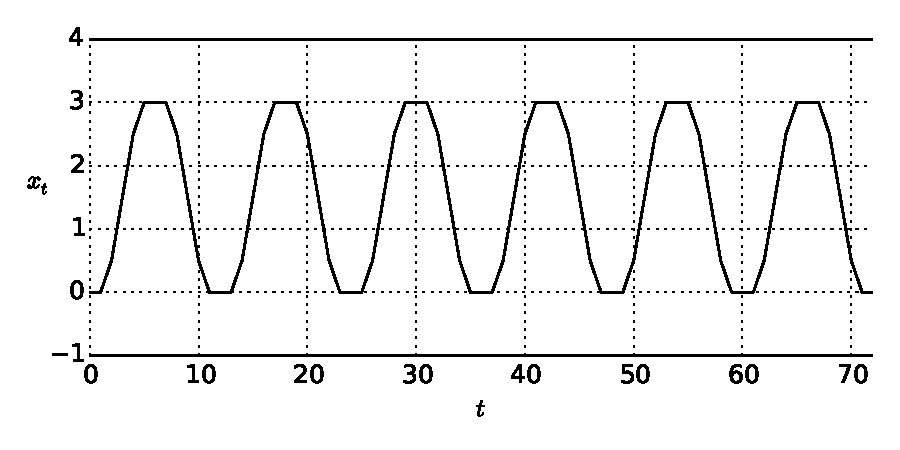
\includegraphics[width=1\textwidth]{img/osc-step.pdf}
    \caption{Oscillatory discrete time series.}
    \label{fig:osc-step}
\end{figure}

Taking the difference between successive values $x_t$ and $x_{t+1}$ 
as symbols in an alphabet this sequence belongs to the regular language

\[
    \left[
        \left[+0\right]^*
        \left[+\tfrac{1}{2}\right]^+
        \left[+1\right]^*
        \left[+\tfrac{1}{2}\right]^+
        \left[+0\right]^*
        \left[-\tfrac{1}{2}\right]^+
        \left[-1\right]^*
        \left[-\tfrac{1}{2}\right]^+
    \right]^*
\]

which is recognized by the \ac{DFA} in Figure (\ref{fig:cyclic-dfa}).

\begin{figure}[H]
    \centering
    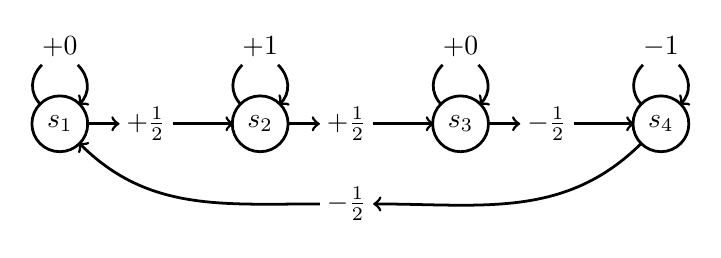
\begin{tikzpicture}
        \tikzstyle{every circle node}=[circle,draw,minimum size=20pt,line width=1pt];
        \node[circle] (s1) {$s_1$};
        \node[textbox,font=\normalsize,above=10pt of s1] (s1s1) {$+0$};
        \node[textbox,font=\normalsize,right=10pt of s1] (s1s2) {$+\frac{1}{2}$};
        
        \node[circle,right=20pt of s1s2] (s2) {$s_2$};
        \node[textbox,font=\normalsize,above=10pt of s2] (s2s2) {$+1$};
        \node[textbox,font=\normalsize,right=10pt of s2] (s2s3) {$+\frac{1}{2}$};
        
        \node[circle,right=20pt of s2s3] (s3) {$s_3$};
        \node[textbox,font=\normalsize,above=10pt of s3] (s3s3) {$+0$};
        \node[textbox,font=\normalsize,right=10pt of s3] (s3s4) {$-\frac{1}{2}$};
        
        \node[circle,right=20pt of s3s4] (s4) {$s_4$};
        \node[textbox,font=\normalsize,above=10pt of s4] (s4s4) {$-1$};
        \node[textbox,font=\normalsize,below=10pt of s2s3] (s4s1) {$-\frac{1}{2}$};        

        \draw[line width=1pt,shorten >= -1pt, shorten <= -1pt] (s1) to[in=225,out=135] (s1s1);
        \draw[->,line width=1pt,shorten >= -1pt, shorten <= -1pt] (s1s1) to[in=45,out=315] (s1);
        \draw[->,line width=1pt,shorten >= -1pt, shorten <= -1pt] (s1) to (s1s2);
        \draw[->,line width=1pt,shorten >= -1pt, shorten <= -1pt] (s1s2) to (s2);

        \draw[line width=1pt,shorten >= -1pt, shorten <= -1pt] (s2) to[in=225,out=135] (s2s2);
        \draw[->,line width=1pt,shorten >= -1pt, shorten <= -1pt] (s2s2) to[in=45,out=315] (s2);
        \draw[->,line width=1pt,shorten >= -1pt, shorten <= -1pt] (s2) to (s2s3);
        \draw[->,line width=1pt,shorten >= -1pt, shorten <= -1pt] (s2s3) to (s3);

        \draw[line width=1pt,shorten >= -1pt, shorten <= -1pt] (s3) to[in=225,out=135] (s3s3);
        \draw[->,line width=1pt,shorten >= -1pt, shorten <= -1pt] (s3s3) to[in=45,out=315] (s3);
        \draw[->,line width=1pt,shorten >= -1pt, shorten <= -1pt] (s3) to (s3s4);
        \draw[->,line width=1pt,shorten >= -1pt, shorten <= -1pt] (s3s4) to (s4);

        \draw[line width=1pt,shorten >= -1pt, shorten <= -1pt] (s4) to[in=225,out=135] (s4s4);
        \draw[->,line width=1pt,shorten >= -1pt, shorten <= -1pt] (s4s4) to[in=45,out=315] (s4);
        \draw[->,line width=1pt,shorten >= -1pt, shorten <= -1pt] (s4) to[in=0,out=225] (s4s1);
        \draw[->,line width=1pt,shorten >= -1pt, shorten <= -1pt] (s4s1) to[in=315,out=180] (s1);
    \end{tikzpicture}
    \caption{4 state cyclic \ac{DFA}.}
    \label{fig:cyclic-dfa}
\end{figure}

The natural probabilistic generalization of this \ac{DFA} is a \ac{HMM}
with a cyclic transition structure and parametric emission distributions replacing
discrete symbols, Figure (\ref{fig:cyclic-hmm}). 

\begin{figure}[H]
    \begin{tikzpicture}
        \tikzstyle{every circle node}=[circle,draw,minimum size=20pt,line width=1pt];
        \node[circle] (s1) {$s_1$};
        \node[textbox,below=20pt of s1] (e1) {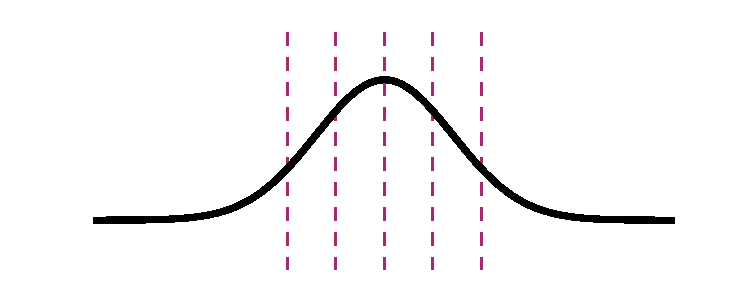
\includegraphics[width=0.25\textwidth]{img/gauss/gauss-0.pdf}};
        \node[textbox,font=\normalsize,above=20pt of s1] (s1s1) {$P(s_1|s_1)$};
        \node[textbox,font=\normalsize,right=10pt of s1] (s1s2) {$P(s_2|s_1)$};
        
        \node[circle,right=10pt of s1s2] (s2) {$s_2$};
        \node[textbox,below=20pt of s2] (e2) {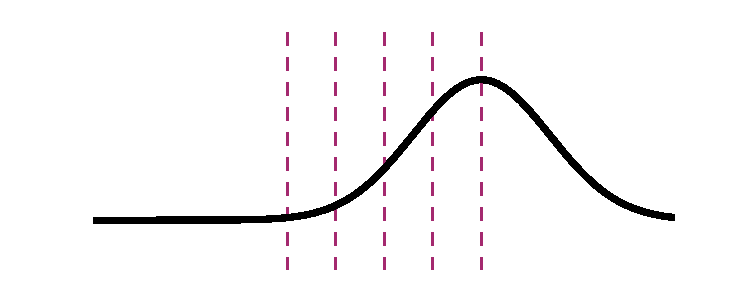
\includegraphics[width=0.25\textwidth]{./img/gauss/gauss-1.pdf}};
        \node[textbox,font=\normalsize,above=20pt of s2] (s2s2) {$P(s_2|s_2)$};
        \node[textbox,font=\normalsize,right=10pt of s2] (s2s3) {$P(s_3|s_2)$};
        
        \node[circle,right=10pt of s2s3] (s3) {$s_3$};
        \node[textbox,below=20pt of s3] (e3) {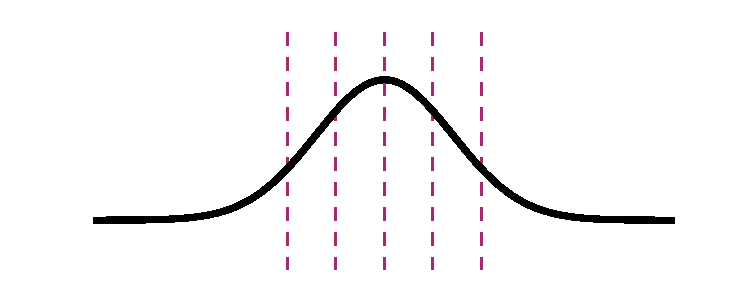
\includegraphics[width=0.25\textwidth]{./img/gauss/gauss-0.pdf}};
        \node[textbox,font=\normalsize,above=20pt of s3] (s3s3) {$P(s_3|s_3)$};
        \node[textbox,font=\normalsize,right=10pt of s3] (s3s4) {$P(s_4|s_3)$};
        
        \node[circle,right=10pt of s3s4] (s4) {$s_4$};
        \node[textbox,below=20pt of s4] (e4) {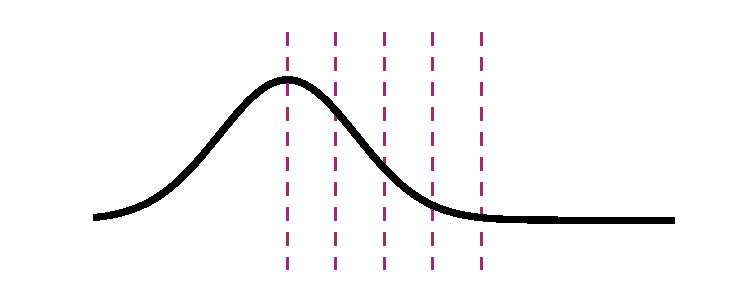
\includegraphics[width=0.25\textwidth]{./img/gauss/gauss-neg1.pdf}};
        \node[textbox,font=\normalsize,above=20pt of s4] (s4s4) {$P(s_4|s_4)$};
        \node[textbox,font=\normalsize,above=40pt of s2s3] (s4s1) {$P(s_1|s_4)$};        

        \draw[line width=1pt,shorten >= -1pt, shorten <= -1pt] (s1) to[in=225,out=135] (s1s1);
        \draw[->,line width=1pt,shorten >= -1pt, shorten <= -1pt] (s1s1) to[in=45,out=315] (s1);
        \draw[->,line width=1pt,shorten >= -1pt, shorten <= -1pt] (s1) to (s1s2);
        \draw[->,line width=1pt,shorten >= -1pt, shorten <= -1pt] (s1s2) to (s2);
        \draw[->,line width=1pt,shorten >= -1pt, shorten <= -1pt] (s1) to (e1);

        \draw[line width=1pt,shorten >= -1pt, shorten <= -1pt] (s2) to[in=225,out=135] (s2s2);
        \draw[->,line width=1pt,shorten >= -1pt, shorten <= -1pt] (s2s2) to[in=45,out=315] (s2);
        \draw[->,line width=1pt,shorten >= -1pt, shorten <= -1pt] (s2) to (s2s3);
        \draw[->,line width=1pt,shorten >= -1pt, shorten <= -1pt] (s2s3) to (s3);
        \draw[->,line width=1pt,shorten >= -1pt, shorten <= -1pt] (s2) to (e2);

        \draw[line width=1pt,shorten >= -1pt, shorten <= -1pt] (s3) to[in=225,out=135] (s3s3);
        \draw[->,line width=1pt,shorten >= -1pt, shorten <= -1pt] (s3s3) to[in=45,out=315] (s3);
        \draw[->,line width=1pt,shorten >= -1pt, shorten <= -1pt] (s3) to (s3s4);
        \draw[->,line width=1pt,shorten >= -1pt, shorten <= -1pt] (s3s4) to (s4);
        \draw[->,line width=1pt,shorten >= -1pt, shorten <= -1pt] (s3) to (e3);

        \draw[line width=1pt,shorten >= -1pt, shorten <= -1pt] (s4) to[in=225,out=135] (s4s4);
        \draw[->,line width=1pt,shorten >= -1pt, shorten <= -1pt] (s4s4) to[in=45,out=315] (s4);
        \draw[->,line width=1pt,shorten >= -1pt, shorten <= -1pt] (s4) to[in=0,out=135] (s4s1);
        \draw[->,line width=1pt,shorten >= -1pt, shorten <= -1pt] (s4s1) to[in=45,out=180] (s1);
        \draw[->,line width=1pt,shorten >= -1pt, shorten <= -1pt] (s4) to (e4);
    \end{tikzpicture}
    \caption{4 state \ac{CHMM}.}
    \label{fig:cyclic-hmm}
\end{figure}

\section{Advantages}
This basic, and surprisingly simple model is elaborated upon in various ways to solve a 
number of synthetic and real world tasks related to motion recognition in the following chapters.
As well as inherently capturing the repetitive nature of exercise, a \ac{CHMM} with $K$ 
states only has $O(K)$ transition parameters\footnote{A \ac{CHMM} with $K$ states has 
exactly $2K$ transition parameters.} unlike a \ac{HMM} in which every state can transition
to every other state which has $O(K^2)$ transition parameters. 
This reduction in parameters should require less data to estimate, 
and reduces the computational complexity of typical inference tasks such as 
filtering, smoothing, and decoding from $O(TK^2)$ to $O(TK)$.

\chapter{Synthetic experiments with Hidden Markov Model}
This chapter describes several synthetic experiments carried out utilizing the models and
inference procedures described in the previous Chapters. The focus on synthetic data
is primarily intended as a demonstration and exploration of model aptitude. Experiments
with real world data are presented in the following chapters.

\section{The Trick Coin}
The \emph{trick coin} is a classic \ac{HMM} problem as it is described exactly
by the \ac{HMM} generative story. In this scenario there are two coins, one fair,
and the other biased to come up tails with significantly higher probability than heads. 
A sequence of flip outcomes is observed, however at each time step the flipper chooses
to swaps coins, replacing the fair coin with the biased coin or vice versa with some probability. 
This scenario can be modeled by an \ac{HMM} in which the latent
states represent the coin being used, the observations the observed outcomes, and
the state transitions the probability of swapping coins.
\\\\
A single sequence of 500 flips is observed, to which the parameters of a \ac{HMM} is fit using 
either the collapsed Gibbs sampler or standard the standard \ac{EM}
\footnote{Application of \ac{EM} to \acp{HMM} is commonly also referred to as 
the Baum-Welch algorithm.} 
estimation method. 
The resulting \ac{HMM}'s performance was assessed on two tasks. 1.) Inferring
the coin being used at each time of the training sequence, and 2.) Discriminating between an
out of sample sequence of flips drawn from the two coin switching process or a single coin with the 
same expected value as the trick coin.
\\\\
For the first task, the \ac{HMM} fit with the collapsed Gibbs sampling performed quite well,
and the \ac{MAP} state sequence closely aligned with the true state sequence. 
On the other hand the \ac{HMM} fit with \ac{EM} typically only utilized a single state 
and was therefore unable to distinguish between actual states in a better than random fashion,
Figure (\ref{fig:trick-coin-states}).

\begin{figure}[H]
    \centering
    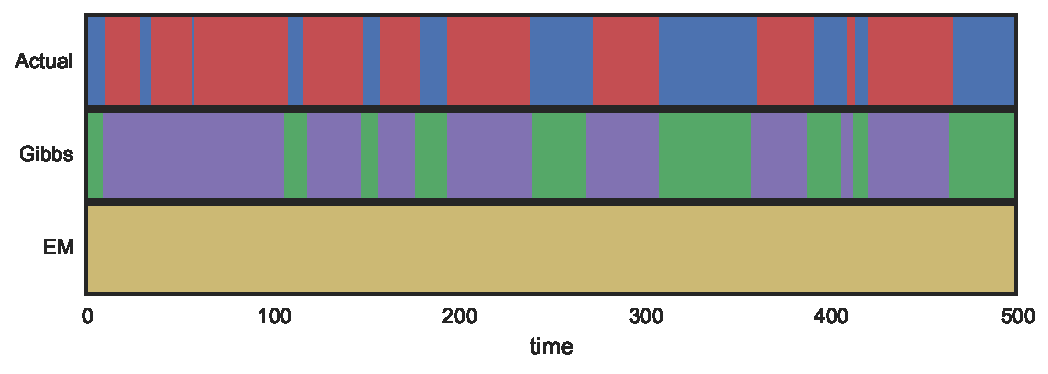
\includegraphics[width=1\textwidth]{img/trick_coin_states.pdf}
    \caption{Actual state sequence and example inferred state sequences from the 
    \ac{HMM} fit with Gibbs sampling and \ac{EM}. The \ac{HMM} fit with \ac{EM}
    only uses a single state to model the observed sequence.}
    \label{fig:trick-coin-states}
\end{figure}

For the second task 500 $(\seq{x}{1}{T}^{\text{trick}}, \seq{x}{1}{T}^\text{single})$ pairs 
of sequences were generated. The ability of each model to discriminate (by comparing likelihoods) 
is assessed for each pair. This same experiment was repeated 25 times using a different single 
training sequence and pairs of testing sequences. Again, the \ac{HMM} fit with Gibbs sampling
significantly outperformed the \ac{HMM} fit with \ac{EM}, Figure (\ref{fig:trick-coin-disc}).

\begin{figure}[H]
    \centering
    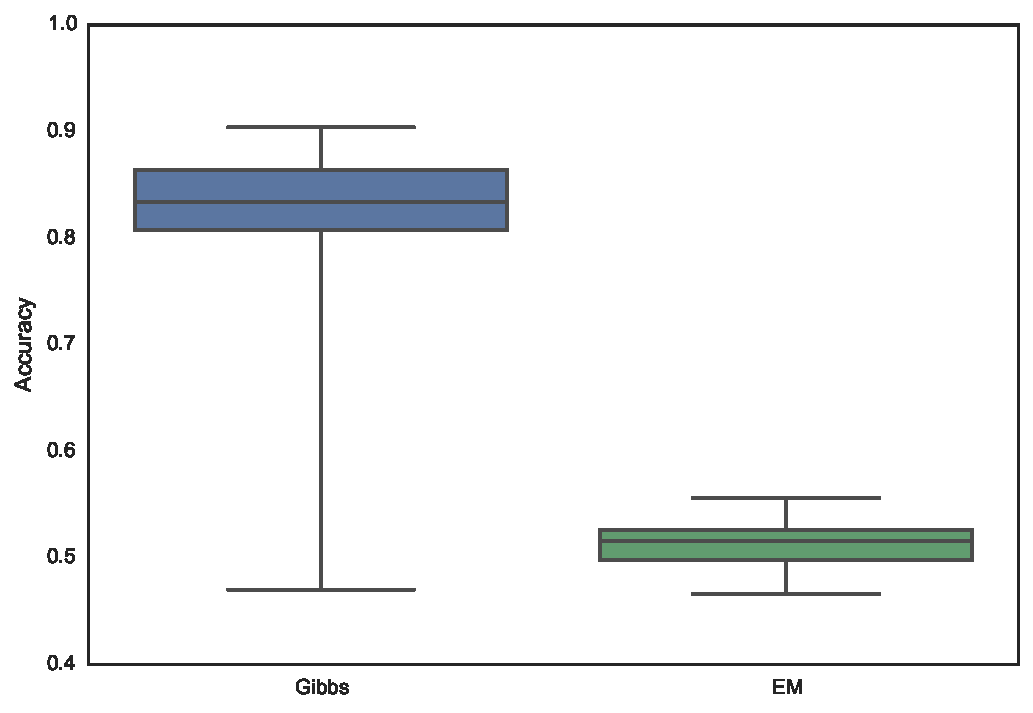
\includegraphics[width=1\textwidth]{img/trick_coin_disc_accuracy.pdf}
    \caption{Accuracy for the trick coin discriminative task. Whiskers 
    depict the maximum and minimum values.}
    \label{fig:trick-coin-disc}
\end{figure}

\section{Learning to Segment Repetitive Sequences}
Having demonstrated the effectiveness of the collapsed Gibbs sampling approach, 
this Section demonstrates the ability of the \ac{CHMM} to utilize its repetitive 
latent structure in an artificial segmentation task. To do so sequences were generate by
embedding a recurrent sequence between two constant sequences and adding Gaussian random noise.
In particular a example sequence is generated from the following distribution.

\begin{align*}
    t_1 & \sim 100 \cdot \Beta(5, 5) + 10 \\
    t_2 & \sim 100 \cdot \Beta(5, 5) + 10 + t_1 \\
    t_3 & \sim 100 \cdot \Beta(5, 5) + 10 + t_2 \\
    \epsilon_t & \sim \Norm(0, 1/2),\; t = 1,\ldots,t_3 \\
    x_t &= \epsilon_t,\; t=1,\ldots,t_1 \\
    x_t &= \sin(t) + \epsilon_t,\; t=t_1+1,\ldots,t_2 \\
    x_t &= \epsilon_t,\; t=t_2 + 1,\ldots,t_3\\
\end{align*}

A model for segmenting such sequences must distinguish between the recurrent portion,
$\seq{x}{t_1+1}{t_2}$, and the constant portions, $\seq{x}{1}{t_1}$, $\seq{x}{t_2+1}{t_3}$.
More formally, each timestep $x_t$ in the sequence is annotated with a tag $a_t \in \{I, O\}$
denoting whether the sequence is \emph{in} ($I$), or \emph{out} ($O$) of the repetitive portion
of the sequence at time $t$. The annotation is similar to the BIO (begin/in/out) representation
commonly used in \ac{NLP} chunking applications \cite{ramshaw-bio}.
\\\\ 
Rather than using these annotations within the learning procedure, for example to learn a 
discriminative classifier, an unsupervised approach is taken, in which only the raw sequence 
is available during training. Thus the ability to discover structure in the time series rests 
entirely on a priori structure built into the model itself.
\\\\
To capture this structure the prior over transition matrices (a Dirichlet distribution for each row) 
is split into three regime blocks. The first and third block corresponds to a standard \ac{HMM}
in which each state may transition to every other state, the \emph{out} portions of the sequence. 
The second block corresponds to the \ac{CHMM} structure in which states transition
only to themselves or their successor states, the \emph{in} portion of the sequence.
To allow movement between these blocks transitions are added from each state in the first block
to the start state of the second block, and from the final state of the second block to each state
in the third block. Diagrammatically this results in the structure depicted below.

\begin{align*}
    \bm{\alpha} &= \left[\begin{array}{c | c | c} 
        F & A_1 & \bm{0} \\\hline 
        \bm{0} & S & A_2 \\\hline 
        \bm{0} & \bm{0} & F
    \end{array}\right] \\
    F &= \left[\begin{array}{c c c} 
        \alpha_0 & \cdots & \alpha_0 \\ 
        \vdots   &        & \vdots \\
        \alpha_0 & \cdots & \alpha_0 
    \end{array}\right] &
    S &= \left[\begin{array}{c c c c c}
        \alpha_3 & \alpha_4 & 0        & \cdots   & 0        \\
        0        & \alpha_3 & \alpha_4 & \ddots   & \vdots   \\
        \vdots   & \ddots   & \ddots   & \ddots   & 0        \\
        0        & \cdots   & 0        & \alpha_3 & \alpha_4 \\
        \alpha_4 & 0        & \cdots   & 0        & \alpha_3
    \end{array}\right] \\
    A_1 &= \left[\begin{array}{c c c c} 
        \alpha_1 & 0      & \cdots & 0 \\ 
        \vdots   & \vdots &        & \vdots \\
        \alpha_1 & 0      & \cdots & 0        
    \end{array}\right] &
    A_2 &= \left[\begin{array}{c c c} 
        0        & \cdots & 0 \\ 
        \vdots   &        & \vdots \\
        0        & \cdots & 0 \\ 
        \alpha_2 & \cdots & \alpha_2
    \end{array}\right]
\end{align*}

Here the $\alpha_i$ terms are parameters of a prior on transitions from

\begin{align*}
    \alpha_0: & \text{ an \emph{out} state to an \emph{out} state,}\\
    \alpha_1: & \text{ an \emph{out} state to an \emph{in} state,}\\
    \alpha_2: & \text{ an \emph{in} state to an \emph{out} state,}\\
    \alpha_3: & \text{ an \emph{in} state to itself,}\\
    \alpha_4: & \text{ an \emph{in} state to its succesor \emph{in} state.}\\
\end{align*}

Using just 2 sample sequences and the above described prior structure with
1 \emph{out} state and 5 \emph{in} states allows the collapsed Gibbs sampler
to discover highly accurate segmentations, Figure (\ref{fig:artificial-segmentation-struct}),
in a completely unsupervised manner. To demonstrate the necessity for the prior
and rule out the possibility that the model is doing something uninteresting such
as modeling differences in variance within the distinct regimes, the same experiment
was repeated with a standard \ac{HMM} with two states. In this case the model is completely
unable to discover any interesting structure in the sequence, 
Figure (\ref{fig:artificial-segmentation-flat}).

\begin{figure}[H]
    \centering
    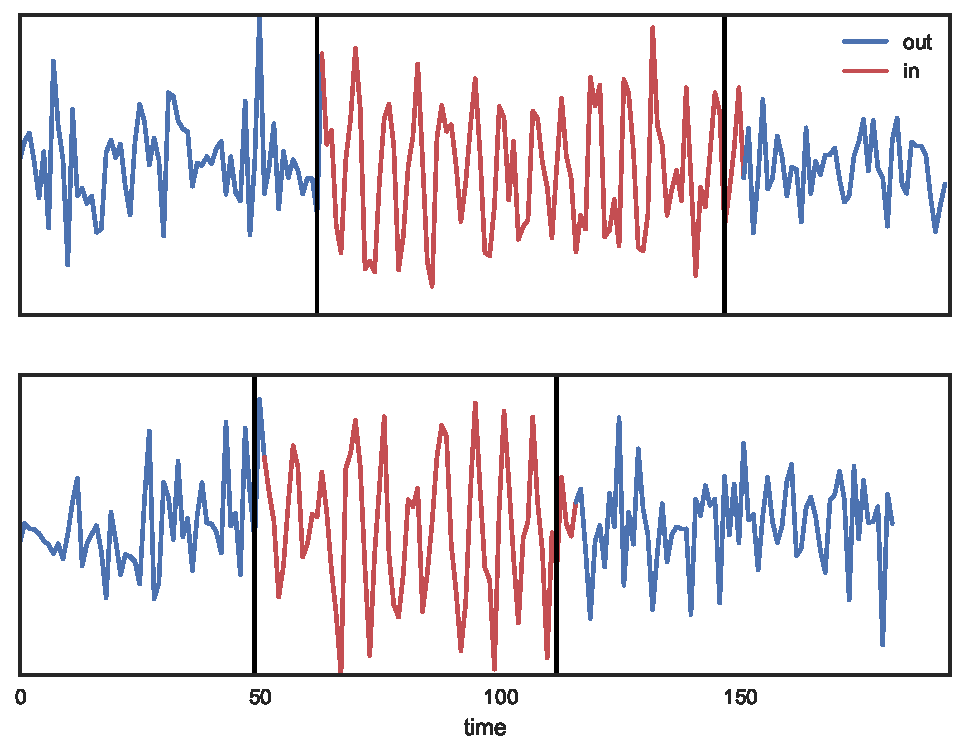
\includegraphics[width=1\textwidth]{img/artificial-segment-output-struct.pdf}
    \caption{Unsupervised segmentation by a \ac{HMM} with structured prior.}
    \label{fig:artificial-segmentation-struct}
\end{figure}

\begin{figure}[H]
    \centering
    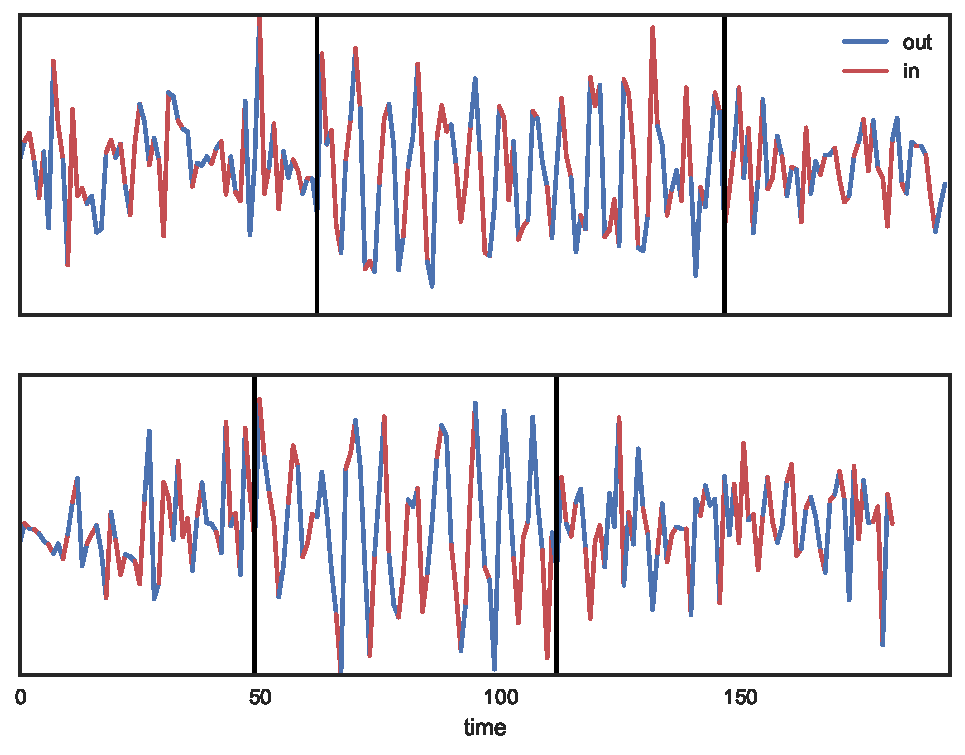
\includegraphics[width=1\textwidth]{img/artificial-segment-output-flat.pdf}
    \caption{Unsupervised segmentation by a \ac{HMM} with 2 states.}
    \label{fig:artificial-segmentation-flat}
\end{figure}

\section{Clustering Sequences}
The final synthetic experiment explores the Bayesian nonparametric approach outlined in 
Section \ref{sec:mohmms} for the purpose of sequence clustering. As ground truth clusters
the following four recurrent functions are used.

\begin{align*}
    f_1(t) &= \sin(t) & 
    f_3(t) &= \max(-2, \min(2, \tan(t/4))) \\
    f_2(t) &= \sin(t) + \sin(t/2) &
    f_4(t) &= \max(0, 2 \cos(t/ 4))
\end{align*}

An example sequences is then generated from the following process.

\begin{align*}
    t_0 & \sim \Unif({0, \ldots, 200}) \\
    t_1 & \sim \Geom(1/10) + 50 + t_0 \\
    \epsilon_t & \sim \Norm(0, 1/2) \\
    x_t &= f_k(t) + \epsilon_t,\; t=t_0,\ldots,t_1.
\end{align*}

This procedure is repeated 10 times for each $k \in \{1,2,3,4\}$ resulting in 40
total training sequences.
\\\\
Two clustering approaches are considered. The first utilizes standard \acp{HMM}
as the base distribution and the second uses \acp{CHMM} as the base distribution.
The experiment is repeated 10 times and the resulting clusterings are compared using 
\ac{AMI} \cite{ami}, a version of Mutual Information corrected to adjust for chance agreements. 
Figure (\ref{fig:artificial-cluster-metrics}) shows that as well as increased performance,
in terms of \ac{AMI}, the Dirichlet Process with \ac{CHMM} base distributions finds
the correct number of clusters in 80\% of experiments. This is in contrast to the standard
\ac{HMM} which is unable to find the actual number of clusters in any of the experiments.

\begin{figure}[H]
    \centering
    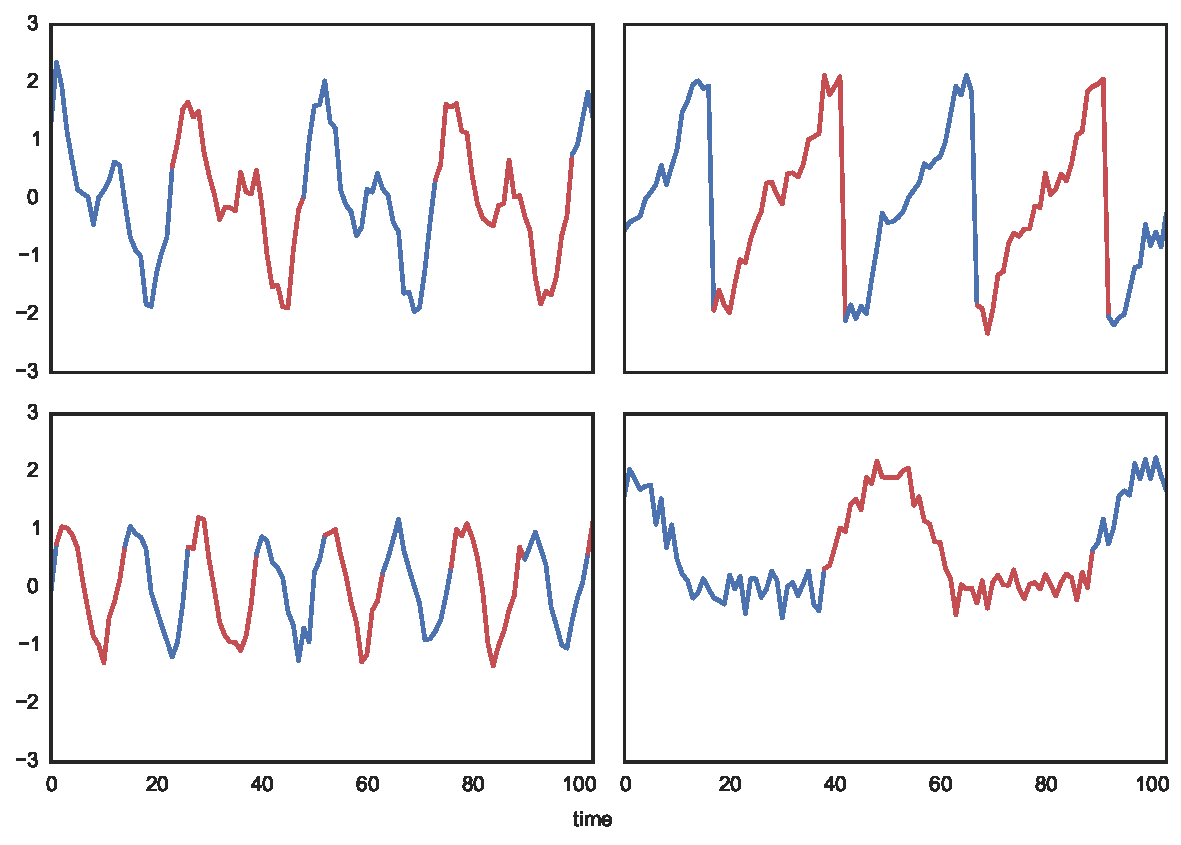
\includegraphics[width=0.8\textwidth]{./img/artificial-clusters.pdf}
    \caption{Example from each cluster and recurrent structure
    discovered by the DP mixture of HMMs with structured prior.}
    \label{fig:artificial-clusters}
\end{figure}

\begin{figure}[H]
    \centering
    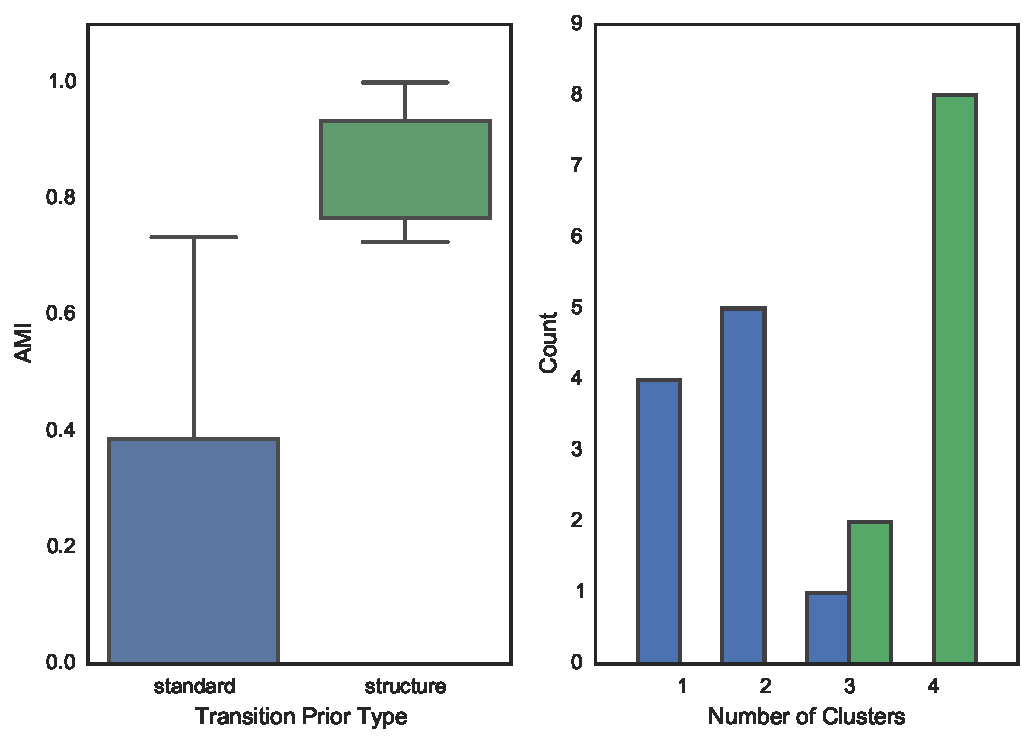
\includegraphics[width=\textwidth]{./img/artificial-cluster-results.pdf}
    \caption{Results from clustering artificial sequences. Comparison of 
    Adjusted mutual information and number of discovered clusters with (green) and without (blue)
    structured transition prior.}
    \label{fig:artificial-cluster-metrics}
\end{figure}


\chapter{Segmented Exercise Classification}
An obvious precursor to classifying each timestep of an entire routines is to classify the hand segmented
exercises into 1 of $K$ mutually exclusive exercise classes. This task is significantly easier than
than the full routine classification task since several simplifying assumptions can be made. First,
we can assume each sequence belongs to a single class. Second, we can assume each class is approximately 
equally likely a priori and avoid dealing with the class imbalance problem that arises when working with
full routines, which are overwhelmingly dominated by \emph{rest}.

\section{Setup}
For training and evaluation purposes we used a random train/test split of the
available data (approximately 70\% of the data was used for training and the remaining
30\% was used for testing) randomized over users. Keeping the set of users in the train and test 
disjoint is particularly important as it mimics the situation one would actually encounter
if deploying such a system. The same train/test split was used for all segment classification
experiments. Classifier hyperparameters were set using grid search performed on an analogous 
split of the training data. Table (\ref{table:segment-dataset}) summarizes the splits.

\begin{table}[ht]
    \centering
    \begin{tabular}{l r r}\hline
    & \textbf{Train} &\textbf{Test} \\\hline
    Users & 85 & 37\\
    Classes & 50 & 50\\
    Activities & 3364 & 1382\\
    Repetitions & 28476 & 12396\\
    Minutes of Data & 1247 & 557\\
    \end{tabular}
    \caption{Summary of segment classification dataset.}
    \label{table:segment-dataset}
\end{table}

\section{Models}
The proposed \ac{CHMM} was compared to a Structured Perceptron \cite{perceptron-collins}
and a strong performing system heavily influenced from the activity recognition literature \cite{ms-activity}. 
As only sequences with a single label are considered in this experiment, a voting procedure is used
to aggregate predictions for individual time steps to produce the final classification for both
the Random Forest and Structured Perceptron. In some sense this gives an unfair advantage to these
models as in a real world activity classification setting, one would not a priori have knowledge of
the bounds (segmentation) over which to aggregate votes.

\subsection{Baseline from Literature}
Decomposition of a temporal classification problem into a series 
of fixed size iid decisions is a common approach to activity recognition
in the literature. \cite{ms-activity} first derive a series of standard features
from the raw sensor data, and then apply a \ac{SVM} to fixed size windows in a similar problem. 
Significantly better results were obtained on the data considered here using a Random Forest 
rather than a \ac{SVM} and only the former is reported here. This discrepancy is likely due 
to \cite{ms-activity} utilizing a number of heuristic feature partitioning schemes which were 
not able to be replicated in this work.
\\\\
The following features were computed over 4 second windows (60 timesteps)
for each of the 3 accelerometer and 3 gyroscope axis:
\begin{itemize}[nosep]
    \item The number of peaks in the autocorrelation function.
    \item The height of the first peak of the autocorrelation function after crossing zero.
    \item The maximum value of the autocorrelation function.
    \item The mean of the signal.
    \item The standard deviation of the signal.
    \item The norm of the signal.
    \item The magnitude of the power specturm summed across 10 linearly spaced bands.
\end{itemize}
The free software scikit-learn \cite{scikit-learn} was used
to estimate parameters if the random forest. Grid search was performed 
over the following hyper-parameters:\footnote{
Best performing settings on the validation set are noted in bold.
}
\begin{itemize}[nosep]
    \item The number of trees in the forest: $(25, 50, \mathbf{100})$.
    \item The minimum number of samples in each leaf node: $(2, \mathbf{5}, 10)$.
    \item The maximum depth of each tree: $(10, 20, \mathbf{none})$.
    \item The maximum number of features considered for each split: $(\mathbf{\sqrt{d}}, all)$.
    \item The spit evaluation function: \textbf{Gini impurity} or information gain.
\end{itemize}

\subsection{Structured Perceptron}
The Structured Perceptron is a discriminative analog of a \ac{HMM}. 
It is worth noting this statement is somewhat tenuous, and it could 
be considered more appropriate to say this is only true of the closely 
related \ac{CRF}, which models $P(Y|X)$ as opposed to a \ac{HMM} 
which models $P(Y,X)$. Regardless, both are chain structured discriminative 
models which avoid the local normalization problems, \emph{label bias}, associated 
with \acp{HMM} and \acp{MEMM} \cite{lafferty-crf}. 
\\\\
Despite avoiding the label bias problem, the gradient based algorithms frequently
used for training such models do not easily extend to models with latent varaiables. 
As latent variables offer a significant amount of flexibility this is a potential
drawback for such models.
\\\\
CRFSuite \cite{CRFsuite}, a free structured linear model implementation, was used
for training the Structured Perceptron. \acp{CRF} and Structured Perceptrons
with Passive Aggressive weight updates were also evaluated for several settings of
hyper-parameters. The Averaged Structured Perceptron obtained lower overall 
error on the data considered here. The Averaged Structured Perceptron has no hyperparameters.

\subsection{Mixtures of Cyclic Hidden Markov Models}
The conditional probability of a sequence belonging to one of the 
$K$ exercise classes can be modeled by forming a mixture of \acp{CHMM} 
and calculating the predictive distribution as
\[
    P(k \mid \seq{x}{1}{T}, \seq{y}{1}{T}) \propto P(k)P(\seq{x}{1}{T}, \mid k)
\]
where $P(k)$ is prior probability of exercises $k$. 
In these experiments, $P(k) = 1 / K$ is fixed. Given labeled segments,
parameter estimation of the component \acp{CHMM} can be carried
out independently. Two methods of parameter estimation are considered. 
\\\\
The first method searches for \ac{MAP} parameters using Viterbi Training 
\cite{segmental-kmeans}. This criteria was found to perform slightly better than the 
typical \ac{EM} approach for estimating \ac{HMM} parameters. Recent work 
provides both empirical and theoretical support for this observation, especially when fitting 
highly misspecified models, and/or in cases in which the final performance will be measured using 
the MAP state sequence. For further discussion on this subject we defer the interested reader 
to Sections 7 and 8 of \cite{viterbi-em} as well as \cite{estimate-wrong}.
\\\\
The second method is based on the collapsed block Gibbs sampling approach outlined in Section
\ref{sec:collapsed-sampler}. The MAP sampled assignment is used to produce a point estimate of the parameters.

\section{Results}
Discussion + Results with \emph{rest} as a class.
\begin{table}[ht]
    \centering
    \begin{tabular}{l r r}\hline
    \textbf{Classifier} & \textbf{Train Error} &\textbf{Test Error} \\\hline
    MAP Baseline & 0.957 & 0.963 \\
    Structured Perceptron & 0.319 & 0.402 \\
    Random Forest & 0.003 & \textbf{0.173} \\
    MoHMM (block Gibbs) & 0.152 & 0.225 \\
    MoHMM (Viterbi) & 0.163 & 0.238 \\
    \end{tabular}
    \caption{Segment classification results.}
    \label{table:segment-results}
\end{table}

\chapter{Segmenting Exercises}
The above strong performing baseline has the disadvantage that it requires ground truth
segmentations. The system presented for segmentation in the synthetic experiments section
can perform this segmentation in an unsupervised manner without ground truth annotations.

\chapter{Simultaneous Segmentation and Classification of Exercises}
This chapter focuses on the most difficult case where the time series $\seq{x}{1}{T}$
contains instances of different exercises interleaved with \emph{rest}, i.e., a routine. 
Thus for each time $t = 1,\ldots,T$ there is an associated label 
$a_t \in \{\varnothing\} \cup \{1, \ldots, K\}$ denoting the current activity, and the algorithm
must output a sequence of labels $\seq{\hat{a}}{1}{T}$.
Metrics are a problem here as predicting interleaved periods of rest during an exercise
are extremely harmful to downstream components (like repetition counting and displaying
information about the entire routine), but are only slightly penalized by something like
mean hamming distance. Furthermore one needs to correct for labeling every time step with the 
majority class ($\varnothing$). For these reasons I've mostly been resorting to visual 
inspection. Possible options include:
\\\\
\textbf{Maximal Overlapping Subsequence:} This isn't something I've found a reference for,
but which seems quite reasonable. For each homogeneous region $\seq{a}{t_1}{t_2}$ find the
maximal overlapping predicted subsequence 

\begin{align*}
    \hat{s} &=  
    \arg\max\{t_2^\p - t_1^\p \mid t_1 \le t_1^\p < t_2^\p \le t_2,\; \hat{a}_i = \hat{a}_j,\; t_1^\p \le i,j \le t_2^\p\} \\
    \err(\hat{s}, \seq{a}{t_1}{t_2}) &= t_1^\p - t_1 + \sum_{i=t_1^\p}^{t_2^\p} \1\{\hat{a}_i = a_i\} + t_2 - t_2^\p.
\end{align*}

For example

\[\begin{array}{c c c c c c c c c c c c c c}
    a       &=& [\varnothing,& \varnothing,& 1,& 1,          & 1,& 1,& 1,& \varnothing,& \varnothing,& 2,& 2,& 2] \\
    \hat{a} &=& [\varnothing,& \varnothing,& 1,& \varnothing,& 1,& 1,& 1,& 1,          & \varnothing,& 2,& 2,& 2] \\
    \err    &=& [0,          & 0,          & 1,& 1,          & 0,& 0,& 0,& 1,          & 0,          & 0,& 0,& 0] \\
\end{array}\]

The total error for the entire sequence is then the error of the individual $s$ terms.
\\\\
\textbf{Edit Distance:} Treat each homogeneous region as a single symbol and compute the edit
distance between the resulting ground truth and predicted strings.

\begin{acronym}
    \acro{DBN}{Dynamic Bayesian Network}
    \acro{HMM}{Hidden Markov model}
    \acro{CHMM}{Cyclic Hidden Markov Model}
    \acro{HHMM}{Hierarchical \ac{HMM}}
    \acro{MoHMM}{Mixture of Hidden Markov Models}
    \acro{DFA}{Deterministic Finite State Automaton}
    \acro{PGM}{Probabilistic Graphical Model}
    \acro{CRF}{Conditional Random Field}
    \acro{MEMM}{Maximum Entropy Markov Model}
    \acro{SVM}{Support Vector Machine}
    \acro{MAP}{Maximum a Posteriori}
    \acro{EM}{Expectation Maximization}
    \acro{PCFG}{Probabilistic Context Free Grammar}
    \acro{MCMC}{Markov Chain Monte Carlo}
    \acro{NLP}{Natural Language Processing}
    \acro{AMI}{Adjusted Mutual Information}
\end{acronym}

\bibliographystyle{alpha}
\bibliography{tllake.thesis}

\end{document}
